%\knowledge{beyond worst-case synthesis}
  [Beyond worst-case synthesis|beyond worst-case|bwc]
  {notion,index={beyond worst-case synthesis}}
\knowledge{multiobjective}
  [Multiobjective]
  {notion,index={multiobjective}}
\knowledge{rich behavioural models}
  [Rich behavioural models]
  {notion,index={rich behavioural models}}
\knowledge{percentile queries}
  [Percentile queries]
  {notion,index={percentile queries}}
\knowledge{multidimension quantitative games}
  [Multidimension quantitative games]
  {notion,index={multidimension quantitative games}}
\knowledge{Pareto-optimal strategy}
  [Pareto-optimality]
  {notion,index={Pareto!optimal strategy}}
\knowledge{Pareto frontier}
  {notion,index={Pareto!frontier}}
\knowledge{half-memoryless determinacy}
  {notion,index={determinacy!half-memoryless}}
\knowledge{worst-case guarantees}
  [Worst-case guarantees]
  {notion,index={worst-case guarantees}}


%*** General probabilistic notation ***

\newcommand{\expv}{\mathbf{E}} % EXP. VALUE
\newcommand{\discProbDist}{f} % Discrete prob distribution
\newcommand{\sampleSpace}{S} % Generic sample space
\newcommand{\sigmaAlg}{\mathcal{F}} % Generic sigma-algebra
\newcommand{\probm}{\mathbb{P}} % Generic probability measure, also prob. measure operator
\newcommand{\rvar}{X} % Generic random variable
%\newcommand{\dist}{\mathit{Dist}}

%*** MDP notation ***

\newcommand{\actions}{A} % The set of actions.
\newcommand{\colouring}{c} % the colouring function
\newcommand{\probTranFunc}{\Delta} % Transition function of an MDP
\newcommand{\edges}{E} % Set of edges in an MDP.
\newcommand{\colours}{C} % The set of colours in an MDP.
\newcommand{\mdp}{\mathcal{M}} % A generic MDP. 
\newcommand{\vinit}{v_0} % An initial vertex in an MDP.
\newcommand{\cylProb}{p} % Function assigning probabilities to cylinder sets in 
%the measure construction.
\newcommand{\emptyPlay}{\epsilon} %empty play
\newcommand{\objective}{\Omega} % Qualitative objective
\newcommand{\genColour}{\textsc{c}} % Generic colour
\newcommand{\quantObj}{f} % Generic quantitative objective
\newcommand{\indicator}[1]{\mathbf{1}_{#1}} % In.d RV
\newcommand{\eps}{\varepsilon} % Numerical epsilon
\newcommand{\maxc}{W} % Maximal abs. value of a colour

\newcommand{\winPos}{W_{>0}}
\newcommand{\winAS}{W_{=1}}
\newcommand{\cylinder}{\mathit{Cyl}}

\newcommand{\PrePos}{\text{Pre}_{>0}}
\newcommand{\PreAS}{\text{Pre}_{=1}}

\newcommand{\PreOPPos}{\mathcal{P}_{>0}}
\newcommand{\OPAS}{\mathcal{P}_{=1}}

\newcommand{\safeOP}{\mathit{Safe_{=1}}}
\newcommand{\closed}{\mathit{Cl}}

\newcommand{\reachOP}{\mathcal{V}}
\newcommand{\discOP}{\mathcal{D}}
\newcommand{\valsigma}{\vec{x}^{\sigma}}

\newcommand{\lp}{\mathcal{L}}
\newcommand{\lpdisc}{\lp_{\mathit{disc}}}
\newcommand{\lpmp}{\lp_{\mathit{mp}}}
\newcommand{\lpsol}[1]{\bar{#1}}
\newcommand{\lpmpdual}{\lpmp^{\mathit{dual}}}

\newcommand{\actevent}[3]{\actions^{#1}_{#2,#3}} % Returns #1-th action on the run 

\newcommand{\MeanPayoffSup}{\MeanPayoff^{+}}
\newcommand{\MeanPayoffInf}{\MeanPayoff^{-}}

\newcommand{\mcprob}{M}
\newcommand{\invdist}{\vec{z}}

\newcommand{\hittime}{T}



Up to this chapter, we have mostly been interested in finding strategies that achieve a \emph{single} objective or optimise a \emph{single} payoff function. Our goal here is to discuss what happens when one goes further and wants to build strategies that (i) ensure \emph{several objectives}, or (ii) provide \emph{richer guarantees} than the simple worst-case or expectation ones used respectively in zero-sum games and MDPs. 

Consider case (i). Such requirements arise naturally in applications: for instance, one may want to define a trade-off between the performance of a system and its energy consumption. A model of choice for this is the natural \textit{multidimension} extension of the games of~\cref{4-chap:payoffs}, where we consider weight vectors on edges and combinations of objectives.

In case (ii), we base our study on stochastic models such as MDPs (\cref{5-chap:mdp}). We will notably present how to devise controllers that provide strong guarantees in a worst-case scenario while behaving efficiently on average (based on a stochastic model of its environment built through statistical observations); effectively reconciling the rational antagonistic behaviour of Adam, used in games, with the stochastic interpretation of uncontrollable interaction at the core of MDPs.

Stepping into the ""multiobjective"" world is like entering a jungle: the sights are amazing but the wildlife is overwhelming. Providing an exhaustive account of existing multiobjective models and the latest developments in their study is a task doomed to fail: simply consider the combinatorial explosion of all the possible combinations based on the already non-exhaustive set of games studied in the previous chapters. Hence, our goal here is to guide the reader through his first steps in the jungle, highlighting the specific dangers and challenges of the multiobjective landscape, and displaying some techniques to deal with them. To that end, we focus on models studied in~\cref{2-chap:regular},~\cref{4-chap:payoffs},~\cref{5-chap:mdp} and~\cref{11-chap:counters}, and multiobjective settings that extend them. We favour simple, natural classes of problems, that already suffice to grasp the cornerstones of multiobjective reasoning. 

\paragraph{Chapter outline} In~\cref{12-sec:multiple_dimensions}, we illustrate the additional complexity of multiobjective games and how relations between different classes of games that hold in the single objective case often break as soon as we consider combinations of objectives. 

The next two sections are devoted to the \emph{simplest form} of multiobjective games: games with \emph{conjunctions} of classical objectives. In~\cref{12-sec:mean_payoff_energy}, we present the classical case of multidimension "mean-payoff" and "energy" games, which preserve relatively nice properties with regard to their single-objective counterparts. In~\cref{12-sec:total_payoff_shortest_path}, we discuss the opposite situation of "total-payoff" and "shortest path" games: their nice single-objective behaviour vanishes here.

In the last two sections, we explore a different meaning of \emph{multiobjective} through so-called ""rich behavioural models"". Our quest here is to find strategies that provide several types of guarantees, of different nature, for the same quantitative objective. In~\cref{12-sec:beyond_worst_case}, we address the problem of \emph{"beyond worst-case synthesis"}, which combines the rational antagonistic interpretation of "two-player zero-sum games" with the stochastic nature of "MDPs". We will study the mean-payoff setting and see how to construct strategies that ensure a strict worst-case constraint while providing the highest expected value possible.
In~\cref{12-sec:percentile}, we briefly present \emph{"percentile queries"}, which extend \textit{probability threshold problems} in MDPs to their multidimension counterparts. \todo{Check what I do exactly.} Interestingly, \emph{"randomized strategies"} become needed in this context, whereas up to~\cref{12-sec:percentile}, we only consider "deterministic" strategies as they suffice.

We close the chapter with the usual bibliographic discussion and pointers towards some of the many recent advances in multiobjective reasoning.

\section{From one to multiple dimensions}
\label{12-sec:multiple_dimensions}
For the first part of this chapter, we consider ""multidimension quantitative games"". With regard to the formalism of~\cref{chap:payoffs}, the only change to the arena is the set of colours associated with edges: we now have vectors in $\R^k$ where $k \in \N_{>0}$ is the ""dimension"" of the game. As before, for computational purposes, it makes sense to restrict our colouring to rational numbers, and for the sake of simplicity, we even consider \emph{integers only} without loss of generality.

For the weighted games of~\cref{chap:payoffs}, where a single quantitative objective $f$ is considered, we know that the "value" of the game exists. In most cases, optimal strategies do too, which makes the problems of computing the value and solving the game for a given threshold morally equivalent. In our simple multidimension setting, we focus on \emph{conjunctions} of objectives. Similarly to what we did in the one-dimension case, we will write $f_{\geq \vec{x}}$ with $\vec{x} \in \Q^k$ to define the objective
\[
f_{\geq \vec{x}} = \bigcap_{i = 1}^{k} \left\lbrace \play \in E^\omega \mid f_i(\play) \geq \vec{x}_i\right\rbrace 
\]
where $f_i(\play)$ represents the evaluation of $f$ on the sequence of colours in the $i$-th dimension and $\vec{x}_i$ represents the $i$-th component of vector $\vec{x}$. Hence we consider the natural semantics where we want to satisfy the original objective $f$ component-wise.

\begin{example}
\label{12-ex:MMP}
Consider the simple one-player game in~\cref{12-fig:MultiMP} fitted with the "mean-payoff" objective $\MeanPayoff^-$  (recall that two variants exist depending on the use of lim-sup or lim-inf). \todo{Notation issue should be solved in Benjamin/Petr's chapters. Add ref here.} Let us first recall that in the single-objective case, memoryless strategies suffice to play optimally (\cref{4-thm:mean_payoff_positional}). In this game, such strategies permit to achieve payoffs $(1,-1)$, $(-1,-1)$ and $(-1,1)$. Intuitively, $(-1,-1)$ is not interesting since we can do better with $(1,-1)$ or $(-1,1)$. On the other hand, these two other payoffs are incomparable and thus should not be discriminated a priori. In the multiobjective world, there is usually no total order between the outcomes of a game -- fixing a total order would actually boil down to transforming the game into a one-dimension game -- which is why there is in general no optimal strategy but rather \emph{Pareto-optimal} ones. Intuitively, a strategy is Pareto-optimal if there exists no other strategy yielding a payoff which is as good in all dimensions and strictly better in at least one dimension.
\end{example}

\begin{definition}[""Pareto-optimal strategy""]
Given a $k$-dimension game $\game$ based on the conjunction of $k$ maximising (w.l.o.g.) quantitative objectives $(f_i)_{i=1}^{k}$, a strategy $\sigma$ for Eve is said to be \emph{Pareto-optimal} if it guarantees a payoff $\vec{x} \in \R^k$ such that for all other strategy $\sigma'$ of Eve ensuring payoff $\vec{x}' \neq \vec{x}$, it holds that $\vec{x}_i > \vec{x}'_i$ for some dimension $i \in \{1, \ldots, k\}$.
\end{definition}
 
  
\begin{figure}[tbp]
  \centering
  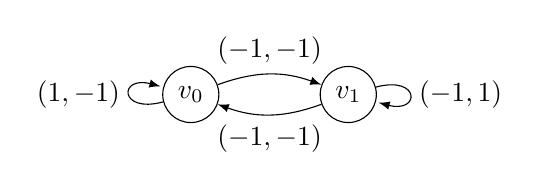
\begin{tikzpicture}[node distance=2cm,>=latex]
    \node[draw,circle](1) {$v_0$};%
    \node[draw,circle,right of=1](2) {$v_1$};%

    \path[->] (1) edge[bend left=20] node[above] {$(-1,-1)$} (2)%
    (2) edge[bend left=20] node[below] {$(-1,-1)$} (1)%
    (1) edge[loop left] node[left] {$(1,-1)$} (1)%
    (2) edge[loop right] node[right] {$(-1,1)$} (2);%

  \end{tikzpicture}
  \caption{A simple multidimension mean-payoff game where Eve needs infinite memory to play (Pareto-)optimally.}
  \label{12-fig:MultiMP}
\end{figure}

The concept of Pareto-optimality has an important consequence on multiobjective problems: the correspondence between solving a threshold problem and computing an optimal strategy that holds in the single-objective case does not carry over. Indeed, one may now be interested in computing the ""Pareto frontier"" consisting of all Pareto  vectors achievable by Eve. This comes at great cost complexity-wise as this frontier may include many points, and in some settings, even an \emph{infinite number of Pareto vectors} (see~\cref{12-sec:percentile} for an example), \todo{Add direct ref when done.} sometimes forcing us to resort to approximation. This requires specific techniques that go beyond the focus of this chapter, hence in the following we mostly discuss the \emph{"threshold problem"}, also referred to as ``solving the game'' for a given threshold vector.

\begin{example}
\label{12-ex:MMP2}
Let us go back to~\cref{12-ex:MMP} and fix objective $\MeanPayoff^{-}_{\geq \vec{x}}$ where $\vec{x} = (0, 0)$. As discussed before, this threshold cannot be achieved by a memoryless strategy. Actually, this is also the case for any \emph{finite-memory} strategy. Indeed, any finite-memory strategy induces an ultimately periodic play, where either (a) the periodic part only visits $v_0$ (resp.~$v_1$), yielding payoff $(1,-1)$ (resp.~$(-1,1)$) thanks to "prefix independence" (\cref{chap:payoffs}), or (b) it visits both in which case the mean-payoff is of the form
\[
\vec{y} = \MeanPayoff^{-}(\play) = \dfrac{a \cdot (1, -1) + 2 \cdot b \cdot (-1, -1) + c \cdot (-1, 1)}{a + 2 \cdot b + c}
\]
where $a, c \in \N$ and $b \in \N_{>0}$. Observe that $\vec{y}_1 + \vec{y}_2 = -4\cdot b / (a + 2 \cdot b + c)$, which is strictly less than zero for any value of the parameters. Hence $\vec{x} = (0, 0)$ is not achievable. Now consider what happens with infinite memory: let $\sigma$ be the strategy of Eve that visits $\ell$ times $v_0$, then $\ell$ times  $v_1$, and then repeats forever with increasing values of $\ell$. The mean-payoff of the resulting play is the limit of the previous equation when $a = c = \ell$ tends to infinity, with $b = 1$: intuitively, the switch between $v_0$ and $v_1$ becomes negligible and the mean-payoff is $\frac{1}{2} \cdot (1,-1) + \frac{1}{2}\cdot(-1,1) = (0, 0)$.
\end{example}

\begin{remark}
While Eve cannot achieve $(0, 0)$ with finite memory, she can achieve (i.e., ensure at least) any payoff $(-\varepsilon, -\varepsilon)$ for $\varepsilon > 0$, using sufficient memory: for instance, by taking $b = 1$ and $a = c = \lceil \frac{1}{\varepsilon} - 1\rceil$ (if $\varepsilon \geq 1$, any strategy works so $a = b = 0$ is fine). In that sense, the payoff $\vec{x} = (0, 0)$ achievable by an infinite-memory strategy can be seen as the supremum of payoffs achievable by finite-memory strategies. Actually, this is exactly how we defined strategy $\sigma$: Eve plays according to an infinite sequence of finite-memory strategies parametrised by $\ell$, such that each strategy of the sequence ensures mean-payoff $(-\varepsilon, -\varepsilon)$, with $\varepsilon \to 0$ when $\ell \to \infty$.
\end{remark}

\begin{example}
\label{12-ex:MMP3}
The reasoning above holds similarly for $\MeanPayoff^{+}$. With finite-memory, the lim-sup variant coincides with the lim-inf one: because the play is \textit{ultimately periodic}, the limit exists. With infinite-memory, Eve can actually achieve the payoff $\vec{x}' = (1, 1)$, witnessing a gap with the lim-inf variant. To do so, she has to play a strategy that alternates between $v_0$ and $v_1$ while staying in each vertex for a sufficiently long period such that the current mean over the corresponding dimension gets close to $1$. Getting these means closer and closer to $1$ and using the lim-sup component-wise then suffices to achieve payoff $\vec{x}'$. For instance, starting in~$v_0$, Eve could choose  $v_1$ 10 times to reach mean $0.9$ on the second dimension, then choose $v_0$ 2189 times to reach mean $0.99$ on the first dimension, and so on. This is in stark contrast to the lim-inf variant, which cannot achieve any payoff $(\varepsilon, \varepsilon)$ for $\varepsilon > 0$ (the Pareto vectors correspond to linear combinations of simple cycles, as hinted before).
\end{example}

\begin{theorem}
\label{12-thm:MMP-Eve}
Multidimension mean-payoff games require infinite-memory strategies for Eve. Furthermore, the lim-inf and lim-sup variants are not equivalent, i.e., their winning regions are in general not identical.
\end{theorem}

This theorem already shows the first signs of our single-objective assumptions crumbling in the multiobjective world: we jump from memoryless determinacy to needing infinite memory, and objectives that were equivalent both in games and MDPs turn out to be different here. Buckle up, as this was only our first step.


\section{Mean-payoff and energy}
\label{12-sec:mean_payoff_energy}
Another well-known equivalence in one-dimension is the one between "mean-payoff" and "energy" games (in the "existential initial credit" form), mentioned in~\cref{chap:payoffs}. The reduction is trivial: Eve has a winning strategy (and an initial credit) in the energy game if and only if she has a strategy to ensure mean-payoff at least equal to zero in the mean-payoff game played over the same arena. Intuitively, the mean-payoff strategy of Eve has to reach a subgame where she can ensure that all cycles formed are non-negative (see "cycle games" in~\cref{chap:payoffs}). The initial credit (which can be as high as Eve wants) offsets the cost of reaching such a subgame as well as the low point of cycles in it (which can be negative but is bounded).

How does it fare in multiple dimensions? The study of "vector games" with "energy semantics" in~\cref{11-chap:counters} gives the following result.

\begin{theorem}
\label{12-thm:MEG}
Solving multidimension energy games is \coNP-complete. Finite-memory strategies are required for Eve and memoryless ones suffice for Adam.
\end{theorem} 

Based on~\cref{12-thm:MMP-Eve} and~\cref{12-ex:MMP2}, it is clear that the aforementioned equivalence holds no more, as mean-payoff games benefit from infinite memory while energy games do not. In~\cref{12-ex:MMP2}, the strategy that achieves $\vec{x} = (0, 0)$ for the mean-payoff does so by switching infinitely often but with decreasing frequency between $v_0$ and $v_1$: the switch becomes negligible in the limit which is fine for the mean-payoff. Still, this would lead the energy to drop below zero eventually, whatever the initial credit chosen by Eve, hence showing why the reduction does not carry over.


\subsection{Finite memory}

Game-theoretic models are generally used in applications, such as controller synthesis, where one actually wants to \textit{implement} a winning strategy when it exists. This is why "finite-memory" strategies have a particular appeal. Hence it is interesting to study what happens when we restrict Eve to finite-memory strategies in multidimension mean-payoff games. 

We first observe that when both players use finite-memory strategies, the resulting play is ultimately periodic, hence the lim-inf and lim-sup variants coincide (the limit exists) and take the value of the mean over the periodic part.

\begin{proposition}
\label{12-prop:MPSI}
The lim-sup and lim-inf variants of multidimension mean-payoff games coincide under finite-memory, i.e., their winning regions are identical in all games.
\end{proposition}

We now go back to the relationship with energy games. In the following, we write  $\vec{0}$ for the $k$-dimension vector $(0,\ldots{},0)$. When restricting both players to finite memory, we regain the equivalence between mean-payoff and energy games by a natural extension of the argument sketched above for one-dimension games.

\begin{theorem}
\label{12-thm:MPEG-equivalence}
For all arena and initial vertex, Eve has a winning strategy for the existential initial credit multidimension energy game if and only if she has a finite-memory winning strategy for the multidimension mean-payoff game with threshold $\vec{x} = \vec{0}$.
\end{theorem}

\begin{proof}
Let $\arena$ be an arena coloured by integer vectors of dimension $k$ and $v_0$ be the initial vertex. We first consider the left-to-right implication. Assume that Eve has a strategy $\sigma$ and some initial credit $\vec{c}_0 \in \N^k$ such that she wins the energy objective over $\arena$. By~\cref{12-thm:MEG}, we may assume $\sigma$ to be finite-memory and $\mem = (M, m_0, \delta)$ to be its "memory structure". Let $\arena_\sigma$ be the classical product of the arena with this memory structure ($\arena \times \mem$) restricted to the choices made by $\sigma$. We claim that any cycle in $\arena_\sigma$ is non-negative in all dimensions (we simply project paths of $\arena_\sigma$ to $C^\omega$ to interpret them as we do for paths in $\arena$). By contradiction, assume that there exists a cycle whose sum of weights is strictly negative in some dimension. Then the play reaching this cycle and looping in it forever is a play consistent with $\sigma$ that is losing for the energy objective, contradicting the hypothesis. Hence, it is indeed the case that all reachable cycles in $\arena_\sigma$ are non-negative in all dimensions. Thus, $\sigma$ ensures mean-payoff at least equal to zero in all dimensions (for lim-inf and lim-sup variants).

In the opposite direction, assume that $\sigma$ is a finite-memory winning strategy for $\MeanPayoff^{-}_{\geq \vec{0}}$ (or equivalently $\MeanPayoff^{+}_{\geq \vec{0}}$). Using the same argument as before, we have that all cycles in $\arena_\sigma$ are non-negative. Therefore there exists some initial credit $\vec{c}_0 \in \N^k$ such that $\sigma$ satisfies the energy objective. As a trivial bound, one may take initial credit $\vert V\vert \cdot \vert M \vert \cdot W$ in all dimensions, where $\vert V\vert$ is the number of vertices of $\arena$, $\vert M \vert$ the number of memory states of $\mem$, and $W$ is the largest absolute weight appearing in the arena: this quantity bounds the lowest sum of weights achievable under an acyclic path.
\end{proof}

Observe that the finite-memory assumption is crucial to lift mean-payoff winning strategies to the energy game. Intuitively, the reasoning would break for a strategy like the one used in~\cref{12-ex:MMP2} because the memory structure would need to be infinite and $\arena_\sigma$ would actually not contain any cycle but an infinite path of ever-decreasing energy such that no bound on the initial credit could be established.

Also, note that~\cref{12-thm:MPEG-equivalence} makes no mention of the specific variant of mean-payoff used. This is because both players play using finite-memory: Eve by hypothesis and Adam thanks to the equivalence and~\cref{12-thm:MEG}. Hence,~\cref{12-prop:MPSI} applies. To sum up, we obtain the following.

\begin{corollary}
Solving multidimension mean-payoff games under finite-memory is \coNP-complete. Finite-mem\-ory strategies are required for Eve and memoryless ones suffice for Adam.
\end{corollary}


\subsection{Infinite memory}

We now turn to the general case, where Eve is allowed to use infinite memory. By~\cref{12-ex:MMP3}, we already know that lim-sup and lim-inf variants are not equivalent. We will cover the lim-sup case in details and end with a brief overview of the lim-inf one.

\subsection*{Lim-sup variant}

Without loss of generality, we fix the objective $\MeanPayoff^{+}_{\geq \vec{0}}$ (one can always modify the weights in the arena and consider the shifted-game with threshold zero). We have seen in our original example (\cref{12-fig:MultiMP}) that Eve could focus on each dimension independently and alternatively in such a way that in the limit, she obtains the supremum in each dimension. This is the core idea that we will exploit.

\begin{lemma}
\label{12-lem:MMP-Eve}
Let $\arena$ be an arena such that from all vertex $v \in \vertices$ and for all dimension $i$, $1 \leq i \leq k$, Eve has a winning strategy for $\{\play \in E^\omega \mid \MeanPayoff^{+}_{i}(\play) \geq 0\}$. Then, from all vertex $v \in \vertices$, she has a winning strategy for $\MeanPayoff^{+}_{\geq \vec{0}}$.
\end{lemma}

Hence, being able to win in each dimension \textit{separately} suffices to guarantee winning in all dimensions \textit{simultaneously}. Note that the converse is obvious.

\begin{proof}
For each vertex $v \in \vertices$ and dimension $i$, $1 \leq i \leq k$, let $\sigma_i^v$ be a winning strategy for Eve from $v$ for $\{\play \in E^\omega \mid \MeanPayoff^{+}_{i}(\play) \geq 0\}$.

Let $T_{\sigma_i^v}$ be the infinite tree obtained by \textit{unfolding}  $\sigma_i^v$: it represents all plays consistent with this strategy. Formally, such a tree is obtained inductively as follows:
\begin{itemize}
\item The root of the tree represents $v$.
\item Given a node\footnote{Nodes refer to the tree, vertices to the arena.} $\eta$ representing the branch (i.e., prefix of play) $\rho$ starting in vertex $v$ and ending in vertex $v_\eta$, we add children as follows:
\begin{itemize}
\item if $v_\eta \in V_{\text{Eve}}$, $\eta$ has a unique child representing the vertex $\out(e)$ reached through edge $e = \sigma_i^v(\rho)$;
\item otherwise $\eta$ has one child for each possible successor of $v_\eta$, i.e., for each $\out(e)$ such that $e \in E$ and $\ing(e) = v_\eta$.
\end{itemize} 
\end{itemize} 
For $\varepsilon > 0$, we declare a node $\eta$ of $T_{\sigma_i^v}$ to be \textit{$\varepsilon$-good} if the mean over dimension $i$ on the path from the root to $\eta$ is at least $-\varepsilon$ (as usual, we project this path to $C^\omega$ to evaluate it). For $\ell \in \N$, let $\widehat{T}^{i, \ell}_{v, \varepsilon}$ be the tree obtained from $T_{\sigma_i^v}$ by removing all descendants of $\varepsilon$-good nodes that are at depth at least $\ell$: hence, all branches of $\widehat{T}^{i, \ell}_{v, \varepsilon}$ have length at least $\ell$ and their leaves are $\varepsilon$-good.

We first show that $\widehat{T}^{i, \ell}_{v, \varepsilon}$ is a finite tree. By K\"onig's Lemma~\cite{Konig:1936}, we only need to show that every branch is finite. By contradiction, assume it is not the case and there exists some infinite branch. By construction, it implies that this branch contains no $\varepsilon$-good node after depth $\ell$. Thus, the corresponding play $\pi$, which is consistent with $\sigma_i^v$, necessarily has $\MeanPayoff^{+}_{i}(\play) \leq -\varepsilon$. This contradicts the hypothesis that $\sigma_i^v$ is winning for dimension $i$. Hence the tree is indeed finite.

Based on these finite trees, we now build an infinite-memory strategy for Eve that will be winning for the conjunct objective $\MeanPayoff^{+}_{\geq \vec{0}}$:
% \SetKwBlock{Loop}{loop}{EndLoop}
% \RestyleAlgo{plain}
%\vspace{-5mm}
\begin{algorithm}[ht]
$\varepsilon \leftarrow 1$

\Loop{
	\For{$i = 1$ to $k$}{
		Let $v$ be the current vertex, $L$ the length of the play so far.
		
		$\ell \leftarrow \frac{L\cdot W}{\varepsilon}$
		
		Play according to $\sigma_i^v$ until a leaf of $\widehat{T}^{i, \ell}_{v, \varepsilon}$ is reached.
	}
	$\varepsilon \leftarrow \frac{\varepsilon}{2}$
}
\caption{This is an algorithm}
\label{12-algo:not_sure_what_this_does}
\end{algorithm}
% \RestyleAlgo{ruled}

%\vspace{-5mm}
\noindent Recall that $W$ is the largest absolute weight in the game. Consider the situation whenever an iteration of the for-loop ends. Let $M$ be the number of steps the play followed $\sigma_i$ during this loop execution. Then, the mean-payoff in dimension $i$ is at least $\frac{-L\cdot W - M\cdot \varepsilon}{L + M} \geq \frac{-L\cdot W - M\cdot \varepsilon}{M}$. Since $M \geq \frac{L\cdot W}{\varepsilon}$ by definition, we obtain that the mean-payoff in dimension $i$ is at least $-2\cdot \varepsilon$.

Observe that since all trees are finite, we always exit the for-loop eventually, hence $\varepsilon$ tends to zero. Therefore, the supremum mean-payoff is at least zero in all dimensions, which makes this strategy winning for $\MeanPayoff^{+}_{\geq \vec{0}}$.
\end{proof}

This construction is tight in the sense that infinite memory is needed for Eve, as previously proved. For Adam, we show a better situation. The proof scheme will also be the base of the upcoming algorithm.

\begin{lemma}
\label{12-lem:MMP-Adam}
Memoryless strategies suffice for Adam in multidimension lim-sup mean-payoff games.
\end{lemma}

\begin{proof}
The proof works by induction on the number of vertices of the arena. The base case $\vert V\vert = 1$ is trivial. Assume the only vertex belongs to Adam. If there exists a self loop (recall we allow several edges per pair of vertices) which has a negative weight on some dimension, Adam wins by looping on it forever. In the opposite case, he cannot win.

Now assume $\vert V\vert \geq 2$. For $i \in \{1,\ldots,k\}$, let $W^i_{\text{Adam}}$ be the winning region of Adam for the complement of $\{\play \in E^\omega \mid \MeanPayoff^{+}_{i}(\play) \geq 0\}$, i.e., the region where Adam has a strategy to force a strictly negative mean-payoff in dimension $i$ (as studied in \cref{4-sec:MP}). Let $W^{\text{disj}}_{\text{Adam}} = \bigcup_{i = 1}^{k} W^i_{\text{Adam}}$. We have two cases.

First, $W^{\text{disj}}_{\text{Adam}} = \emptyset$. Then, Eve can win all one-dimension games from everywhere and by~\cref{12-lem:MMP-Eve}, she can also win for $\MeanPayoff^{+}_{\geq \vec{0}}$. Thus, Adam has no winning strategy.

Second, $W^{\text{disj}}_{\text{Adam}} \neq \emptyset$. Then, there exists $i \in \{1,\ldots,k\}$ such that $W^i_{\text{Adam}} \neq \emptyset$. In this set, Adam has a memoryless winning strategy $\tau_i$ to falsify objective $\{\play \in E^\omega \mid \MeanPayoff^{+}_{i}(\play) \geq 0\}$ (because one-dimension mean-payoff games are memoryless determined, as proved in~\cref{4-thm:mean_payoff_positional}). This strategy also falsifies $\MeanPayoff^{+}_{\geq \vec{0}}$, hence $W^i_{\text{Adam}}$ is part of the winning region for Adam -- we denote it $W_{\text{Adam}}$, as usual.
By prefix independence of the mean-payoff, the "attractor" $W^{i, \Pre}_{\text{Adam}}= \AttrA(W^i_{\text{Adam}})$ is also part of $W_{\text{Adam}}$. We denote by $\tau_\Pre$ the corresponding attractor strategy of Adam. Moreover, the graph restricted to $\vertices \setminus W^{i, \Pre}_{\text{Adam}}$ constitutes a proper arena $\arena'$.

Let $W'_{\text{Adam}}$ be the winning region of Adam in $\arena'$ (for the original objective $\MeanPayoff^{+}_{\geq \vec{0}}$). The arena $\arena'$ has strictly less vertices than $\arena$ since we removed the non-empty region $W^i_{\text{Adam}}$. Hence we can apply the induction hypothesis: Adam has a memoryless winning strategy $\tau'$ in $W'_{\text{Adam}}$. The region $V \setminus (W^{i, \Pre}_{\text{Adam}} \cup W'_{\text{Adam}})$ is winning for Eve in $\arena'$ by determinacy. But it is also winning in $\arena$, i.e., the original game, since Adam cannot force the play to go in $W^{i, \Pre}_{\text{Adam}}$ from there (otherwise it would be part of the attractor too).

\todo{Would a figure be useful?}

We define the following memoryless strategy for Adam, which we claim is winning from $W_{\text{Adam}} = W^{i, \Pre}_{\text{Adam}} \cup W'_{\text{Adam}}$:
\[
\tau(v) =
\begin{cases}
\tau_\Pre(v) &\text{if } v \in W^{i, \Pre}_{\text{Adam}} \setminus W^{i}_{\text{Adam}},\\
\tau_i(v) &\text{if } v \in W^{i}_{\text{Adam}},\\
\tau'(v) &\text{if } v \in W'_{\text{Adam}}.
\end{cases}
\]
Since we already know that Eve wins from $V \setminus W_{\text{Adam}}$, it remains to prove that $\tau$ is winning from $W_{\text{Adam}}$ to conclude. Consider any play $\pi$ consistent with $\tau$ and starting in $W_{\text{Adam}}$. Two cases are possible. First, the play eventually reaches $W^{i}_{\text{Adam}}$ and Adam switches to $\tau_i$: then prefix independence of the mean-payoff guarantees that Adam wins. Second, the play never reaches $W^{i}_{\text{Adam}}$: then $\pi$ necessarily stays in $\arena'$, and $\tau'$ is winning from $W'_{\text{Adam}}$ in $\arena'$. Therefore, $\tau$ does win from everywhere in $W_{\text{Adam}}$, while being memoryless, which ends the proof.
\end{proof}

We use the core reasoning of this proof to build an algorithm solving multidimension lim-sup mean-payoff games (\cref{12-algo:MMP}). Intuitively, we iteratively remove vertices that are declared losing for Eve because Adam can win on some dimension from them. Such vertices can be computed in "pseudo-polynomial" time using the algorithm presented in~\cref{chap:payoffs}, \todo{I need a label on Subsect. 4.3.4 to cite it precisely.} here dubbed \textsf{SolveOneDimMeanPayoff}, and taking as parameters the arena and the considered dimension. Since removing vertices based on some dimension $i$ may decrease the power of Eve and her ability to win for another dimension $i'$, we need the outer loop: in the end, we ensure that $V'$ contains exactly all the vertices from which Eve has a winning strategy for each dimension. By~\cref{12-lem:MMP-Eve} and the proof of~\cref{12-lem:MMP-Adam}, we know that this is equal to $W_{\text{Eve}}$.

\begin{remark}
\label{12-rmk:properArena}
The restriction $\arena' \downharpoonright V'$ defines a proper arena because $W^i_{\text{Adam}} = \AttrA(W^i_{\text{Adam}})$. Indeed, any vertex $v$ from which Adam can force to reach $W^i_{\text{Adam}}$ also belongs to $W^i_{\text{Adam}}$ by prefix independence of the mean-payoff.
\end{remark}

\begin{algorithm}
 \KwData{Arena $\arena$ with vertices $\vertices$}
 \KwResult{$W_{\text{Eve}}$, the winning region of Eve for $\MeanPayoff^{+}_{\geq \vec{0}}$}
 $\arena' \leftarrow \arena$; $V' \leftarrow V$\;
 \Repeat{$LosingVertices = \text{false}$}{
  $LosingVertices \leftarrow \text{false}$\;
  \For{$i = 1$ to $k$}{
    $W^i_{\text{Adam}} \leftarrow V' \setminus \textsf{SolveOneDimMeanPayoff}(\arena', i)$;\\
    \If{$W^i_{\text{Adam}} \neq \emptyset$}{
    $V' \leftarrow V' \setminus W^i_{\text{Adam}}$\\
    $\arena' \leftarrow \arena' \downharpoonright V'$\tcc*{Restriction of $\arena'$ to $V'$}
    $LosingVertices \leftarrow \text{true}$\;
    }
  }
 }
 \Return $V'$
 \caption{Solver for multidimension lim-sup mean-payoff games}
 \label{12-algo:MMP}
\end{algorithm}

We wrap up with the following theorem.
\begin{theorem}
\label{12-thm:MMPsup}
Solving multidimension lim-sup mean-payoff game is in $\NP \cap \coNP$. Infinite-memory strategies are required for Eve and memoryless ones suffice for Adam. Furthermore, the winning regions can be computed in pseudo-polynomial time, through at most $\vert V \vert \cdot k$ calls to an algorithm solving one-dimension mean-payoff games.
\end{theorem}

\begin{proof}
The correctness of~\cref{12-algo:MMP} follows from~\cref{12-lem:MMP-Eve} and~\cref{12-lem:MMP-Adam}, and its complexity is trivial to assess, using $\textsf{SolveOneDimMeanPayoff}$ as a pseudo-polynomial black-box. The memory bounds follow from~\cref{12-lem:MMP-Eve},~\cref{12-lem:MMP-Adam} and~\cref{12-thm:MMP-Eve}. Hence, only the $\NP \cap \coNP$ membership remains. Recall that the decision problem under study is: given an arena $\arena$ and an initial vertex $v_0$, does $v_0$ belong to $W_{\text{Eve}}$ or not?

We first prove that the problem is in $\NP$. A non-deterministic algorithm guesses the winning region $W_{\text{Eve}}$ containing $v_0$ and witness memoryless strategies $\sigma_i$ for all dimensions (we know that memoryless strategies suffice by~\cref{4-thm:mean_payoff_positional}). Then, it checks for every dimension $i$, for every vertex $v \in W_{\text{Eve}}$, that $\sigma_i$ is winning. This boils down to solving a polynomial number of one-player one-dimension mean-payoff games for Adam over the arenas $\arena_{\sigma_i}$ obtained by fixing $\sigma_i$. As noted in~\cref{chap:payoffs}, \todo{I need a label for Subsect. 4.2.2} it can be done in polynomial time using Karp's algorithm for finding the minimum cycle mean in a weighted digraph~\cite{Karp:1978}. By~\cref{12-lem:MMP-Eve}, we know that if the verification checks out, Eve has a winning strategy in $W_{\text{Eve}}$ for objective $\MeanPayoff^{+}_{\geq \vec{0}}$.

Finally, we prove $\coNP$ membership. The algorithm guesses a memoryless winning strategy $\tau$ for Adam (from $v_0$). The verification then consists in checking that Eve has no winning strategy in the arena $\arena_{\tau}$. This can be done using~\cref{12-algo:MMP}, through $\vert V \vert \cdot k$ calls to \textsf{SolveOneDimMeanPayoff}. In this case however, such calls only need to solve \textit{one-player} one-dimension mean-payoff games for Eve, which again can be done in polynomial time, resorting to Karp's algorithm. Thus, the verification takes polynomial time in total, and $\coNP$ membership follows.
\end{proof}

\subsection*{Lim-inf variant} For the sake of conciseness, we give only a brief sketch. Without loss of generality, we fix the objective $\MeanPayoff^{-}_{\geq \vec{0}}$. We know that infinite-memory strategies are needed for Eve by~\cref{12-thm:MMP-Eve}. Again, things look better for Adam.

\begin{lemma}
\label{12-lem:MPlimInfAdam}
Memoryless strategies suffice for Adam in multidimension lim-inf mean-payoff games.
\end{lemma}

\begin{proof}[Sketch]
We mention the sketch as it is interesting in its own right. Recall that~\cref{chap:payoffs} presented a general recipe, due to Gimbert and Zielonka~\cite{Gimbert&Zielonka:2004,Gimbert&Zielonka:2005}, to prove memoryless determinacy. Clearly, such a recipe cannot work here due to~\cref{12-thm:MMP-Eve}. Still, a similar result by Kopczynski deals with ""half-memoryless determinacy""~\cite{Kopczynski:2006}. This new recipe states that if the objective of Eve is both \textit{prefix independent} and \textit{convex}, then memoryless strategies suffice for Adam. We already know that $\MeanPayoff^{-}_{\geq \vec{0}}$ is prefix independent. An objective is said to be convex if it is closed under combinations (shuffling): if two infinite sequences of colours $\play = \rho_1 \rho_2 \ldots{}$ and $\play' = \rho'_1 \rho'_2 \ldots{}$, with all $\rho_i$, $\rho'_i$ being finite prefixes, belong to the objective, then $\play'' = \rho_1 \rho'_1 \rho_2 \rho'_2 \ldots{}$ does too. Conjunctions of lim-inf mean-payoff are convex, hence the result applies here.
\end{proof}

\begin{remark}
Lim-sup mean-payoff objectives are \textit{not} convex, hence the ad-hoc proof in~\cref{12-lem:MMP-Adam}. Consider the integer sequence $\play = (2)^{5^0} (-4)^{5^1} (2)^{5^2} (-4)^{5^3}\ldots{}$ where the length of the $i$-th sequence of numbers if $5^{i-1}$. One can prove that at the end of each sequence of $2$'s (resp.~$-4$'s), the mean is above (and tends to) $1$ (resp.~is exactly $-3$). Let $\play'$ be the sequence obtained by swapping all $2$'s and $-4$'s. We have $\MeanPayoff^{+}(\play) = \MeanPayoff^{+}(\play') \geq 1$, hence $\play, \play' \in \MeanPayoff^{+}_{\geq 0}$.

Still, by shuffling $\play$ and $\play'$ in one-one alternation, we build $\play'' = 2, -4, 2, -4 \ldots{}$, which is such that $\MeanPayoff^{+}(\play'') = -1$, hence  $\play'' \not\in \MeanPayoff^{+}_{\geq 0}$. Hence lim-sup mean-payoff is not convex.
\end{remark}

Complexity-wise, multidimension lim-inf mean-payoff games look a lot like multidimension energy games, even though we proved they are not equivalent without memory restrictions.

\begin{theorem}
Solving multidimension lim-inf mean-payoff games is $\coNP$-complete. Infinite-memory strategies are required for Eve and memoryless ones suffice for Adam.
\end{theorem}

We already discussed memory through~\cref{12-ex:MMP2} and~\cref{12-lem:MPlimInfAdam}. The $\coNP$-hardness can be shown through a reduction from \textsf{3UNSAT} similar to the one used for existential initial credit multidimension energy games in~\cref{12-exist-hard}. The matching upper bound relies on memoryless strategies being sufficient for Adam, and the capacity to solve one-player instances of multidimension lim-inf mean-payoff games in polynomial time. The latter problem is addressed by reduction to detecting non-negative multi-cycles in graphs (which can be done in polynomial time based on~\cite{Kosaraju&Sullivan:1988}).

\subsection*{Wrap-up} 
We have seen that multidimension mean-payoff games and multidimension energy games behave relatively well. Sure, infinite memory is needed for Eve in general, but complexity-wise, the gap with one-dimension games is small and even non-existent for the lim-sup variant. Furthermore, if we are interested in finite-memory strategies, the equivalence with energy games is preserved. Hence, we may say that both mean-payoff and energy games hold up nicely in the multidimension world.


\section{Total-payoff and shortest path}
\label{12-sec:total_payoff_shortest_path}
In this section, we turn to two other objectives deeply studied in~\cref{chap:payoffs}: we study "total-payoff" and "shortest path" games. We will see that the multidimension setting has dire consequences for both.

\subsection{Total-payoff vs.~mean-payoff}

We start with total-payoff games. As for the mean-payoff, we explicitly consider the two variants, $\TotalPayoff^+$ and $\TotalPayoff^-$, for the lim-sup and lim-inf definitions respectively. While~\cref{chap:payoffs} was written using the lim-sup variant, all results are identical for the lim-inf one in one-dimension games~\cite{Gawlitza&Seidl:2009}.

Recall that one-dimension total-payoff games are memoryless determined and solving them is in $\NP \cap \coNP$ (even in $\UP \cap \coUP$~\cite{Gawlitza&Seidl:2009})\todo{Could be moved in~\cref{chap:payoffs}}. Furthermore, \cref{chap:payoffs} taught us that total-payoff can be seen as a \textit{refinement} of mean-payoff, as it permits to reason about low (using the lim-inf variant) and high (using the lim-sup one) points of partial sums along a play when the mean-payoff is zero. We formalize this relationship in the next lemma, and study what happens in multiple dimensions. 

\begin{lemma}
\label{12-lem:MPTP}
Fix an arena $\arena$ and an initial vertex $v_0 \in \vertices$. Let A, B, C and D denote the following assertions.
%\begin{enumerate}
\begin{itemize}
\item[A.] Eve has a winning strategy for $\MeanPayoff^{+}_{\geq \vec{0}}$.
\item[B.] Eve has a winning strategy for $\MeanPayoff^{-}_{\geq \vec{0}}$.
\item[C.] There exists $\vec{x} \in \Q^{k}$ such that Eve has a winning strategy for $\TotalPayoff^{-}_{\geq \vec{x}}$.
\item[D.] There exists $\vec{x} \in \Q^{k}$ such that Eve has a winning strategy for $\TotalPayoff^{+}_{\geq \vec{x}}$.
\end{itemize}
%\end{enumerate}
In one-dimension games ($k = 1$), all four assertions are equivalent. In multidimension ones ($k > 1$), the only implications that hold are: $C \implies D \implies A$ and $C \implies B \implies A$. All other implications are false in general.
\end{lemma}

\cref{12-lem:MPTP} is depicted in~\cref{12-fig:MPTP}: the only implications that carry over to multiple dimensions are depicted by solid arrows.

\begin{figure}[thb]
\centering
\scalebox{1}{\begin{tikzpicture}[dash pattern=on 10pt off 5,->,>=stealth',double,double distance=2pt,shorten >=1pt,auto,node
    distance=2.5cm,bend angle=45,scale=0.6,font=\normalsize]
    \tikzstyle{p1}=[]
    \tikzstyle{p2}=[draw,rectangle,text centered,minimum size=7mm]
    \node[p1]  (A)  at (-0.5, 0) {$A\colon\:\exists\,\sigma_{A} \models \MeanPayoff^{+}_{\geq \vec{0}}$};
    \node[p1]  (D) at (12.5, 0) {$D\colon\:\exists\, \vec{x} \in \Q^{k},\, \exists\,\sigma_D \models \TotalPayoff^{+}_{\geq \vec{x}}$};
    \node[p1]  (B) at (-0.5, -4) {$B\colon\:\exists\,\sigma_{B} \models \MeanPayoff^{-}_{\geq \vec{0}}$};
    \node[p1]  (C) at (12.5, -4) {$C\colon\:\exists\, \vec{x} \in \Q^{k},\, \exists\,\sigma_C \models \TotalPayoff^{-}_{\geq \vec{x}}$};
    \path
    ;
	\draw[dashed,dash phase =4pt,->,>=stealth,thin,double,double distance=1.5pt] (5.5,0) to (7,0);
	\draw[<-,>=stealth,thin,double,double distance=1.5pt,solid] (4,0) to (5.5,0);
	\draw[dashed,dash phase =4pt,->,>=stealth,thin,double,double distance=1.5pt] (5.5,-4) to (7,-4);
	\draw[<-,>=stealth,thin,double,double distance=1.5pt,solid] (4,-4) to (5.5,-4);
	\draw[<-,>=stealth,thin,double,double distance=1.5pt,solid] (0,-1) to (0,-2);
	\draw[dashed,dash phase =4pt,->,>=stealth,thin,double,double distance=1.5pt] (0,-2) to (0,-3);
	\draw[<-,>=stealth,thin,double,double distance=1.5pt,solid] (12,-1) to (12,-2);
	\draw[dashed,dash phase =4pt,->,>=stealth,thin,double,double distance=1.5pt] (12,-2) to (12,-3);
	\draw[<-,>=stealth,thin,double,double distance=1.5pt,solid] (3,-1) to (5.5,-2);
	\draw[dashed,dash phase =4pt,->,>=stealth,thin,double,double distance=1.5pt] (5.5,-2) to (8,-3);
	\draw[dashed,dash phase =4pt,<-,>=stealth,thin,double,double distance=1.5pt] (3,-3) to (5.5,-2);
	\draw[dashed,dash phase =4pt,->,>=stealth,thin,double,double distance=1.5pt] (5.5,-2) to (8,-1);
\end{tikzpicture}}
\caption{Equivalence between mean-payoff and total-payoff games. Dashed im\-pli\-ca\-tions are only valid in one-dimension games. We use $\sigma \models \Omega$ as a shortcut for ``$\sigma$ is winning from $v_0$ for $\Omega$''.}
\label{12-fig:MPTP}
\end{figure}

\begin{proof}
The implications that remain true in multiple dimensions are the trivial ones. First, satisfaction of the lim-inf version of a given objective clearly implies satisfaction of its lim-sup version by definition. Hence, $B \implies A$ and $C \implies D$. Second, consider a play $\pi \in \TotalPayoff^{-}_{\geq \vec{x}}$ (resp.~$\TotalPayoff^{+}_{\geq \vec{x}}$) for some $\vec{x} \in \Q^{k}$. For all dimension $i \in \{1, \ldots{}, k\}$, the corresponding sequence of mean-payoff infima (resp.~suprema) over prefixes can be \textit{lower-bounded} by a sequence of elements of the form $\frac{\vec{x}_i}{\ell}$ with $\ell$ the length of the prefix. We can do this because the sequence of total-payoffs over prefixes is a sequence of integers: it always achieves the value of its limit $\vec{x}_i$ instead of only tending to it asymptotically as could a sequence of rationals (such as the mean-payoffs). Since $\frac{\vec{x}_i}{\ell}$ tends to zero over an infinite play, we do have that $\pi \in \MeanPayoff^{-}_{\geq \vec{x}}$ (resp.~$\MeanPayoff^{+}_{\geq \vec{x}}$). Thus, $C \implies B$ and $D \implies A$. Along with the transitive closure $C \implies A$, these are all the implications preserved in multidimension games.


In one-dimension games, all assertions are equivalent. As seen before, we have that lim-inf and lim-sup mean-payoff games coincide as memoryless strategies suffice for both players. Thus, we add $A \implies B$, and $D \implies B$ by transitivity. Second, consider a memoryless (w.l.o.g.) strategy $\sigma_B$ for Eve for $\MeanPayoff^{-}_{\geq \vec{0}}$. Let $\play$ be any consistent play. Then all cycles in $\pi$ are non-negative, otherwise Eve cannot ensure winning with $\sigma_B$ (because Adam could pump the negative cycle). Thus, the sum of weights along $\play$ is at all times bounded from below by $-(\vert V\vert-1)\cdot W$ (for the longest acyclic prefix), with $W$ the largest absolute weight, as usual. Therefore, we have $B \implies C$, and we obtain all other implications by transitive closure.

For multidimension games, all dashed implications are false. We only need to consider two of them.
\begin{enumerate}
\item\label{12-lem:MPTP_proof1} To show that implication $D \implies B$ does not hold, consider the Eve-owned one-player game where $V = \{v\}$ and the only edges are two self loops of weights $(1, -2)$ and $(-2, 1)$. Clearly, any finite vector $\vec{x} \in \Q^{2}$ for $\TotalPayoff^{+}_{\geq \vec{x}}$ can be achieved by an infinite-memory strategy consisting in playing both loops successively for longer and longer periods, each time switching after getting back above threshold $\vec{x}$ in the considered dimension. However, it is impossible to build any strategy, even with infinite memory, that satisfies $\MeanPayoff^{-}_{\geq \vec{0}}$ as the lim-inf mean-payoff would be at best a linear combination of the two cycle values, i.e., strictly less than zero in at least one dimension in any case.
\item Lastly, consider the game in~\cref{12-fig:MultiMP} where we modify the weights to add a third dimension with value $0$ on the self loops and $-1$ on the other edges. As already proved, the strategy that plays for $\ell$ steps in the left cycle, then goes for $\ell$ steps in the right one, then repeats for $\ell' > \ell$ and so on, is a winning strategy for $\MeanPayoff^{-}_{\geq \vec{0}}$. Nevertheless, for any strategy of Eve, the play is such that either (i) it only switches between $v_0$ and $v_1$ a finite number of times, in which case the sum in dimension $1$ or $2$ decreases to infinity from some point on; or (ii) it switches infinitely often and the sum in dimension $3$ decreases to infinity. In both cases, objective $\TotalPayoff^{+}_{\geq \vec{x}}$ is not satisfied for any finite vector $\vec{x} \in  \Q^{3}$. Hence, $B \implies D$ is falsified.
\end{enumerate}
All other implications are deduced false as they would otherwise contradict the last two cases by transitivity.
\end{proof}

We see that the relationship between mean-payoff and total-payoff games breaks in multiple dimensions. Nonetheless, one may still hope for good properties for the latter, as one-dimension total-payoff games are in $\NP \cap \coNP$ (\cref{chap:payoffs}). \todo{I need label for Subsect. 4.4.3.} This hope, however, will not last long.

\subsection{Undecidability}

In contrast to mean-payoff games, total-payoff ones become undecidable in multiple dimensions.

\begin{theorem}
\label{12-thm:TPundec}
Total-payoff games are undecidable in any dimension $k \geq 5$.
\end{theorem}

\begin{proof}
We use a reduction from two-dimensional robot games~\cite{Niskanen&Potapov&Reichert:2016}, which were mentioned in~\cref{chap:counters}. They are a restricted case of "configuration reachability" "vector games", recently proved to be already undecidable. They are expressible as follows: $\mathcal{V} = (\mathcal{L} = \{\ell_0, \ell_1\}, T, \mathcal{L}_{\text{Eve}} = \{\ell_0\}, \mathcal{L}_{\text{Adam}} = \{\ell_1\})$ and $T \subseteq \mathcal{L} \times [-M, M]^2\times \mathcal{L}$ for some $M \in \N$. The game starts in configuration $\ell_0(x_0, y_0)$ for some $x_0, y_0 \in \Z$ and the goal of Eve is to reach configuration $\ell_0(0, 0)$.

The reduction is as follows. Given a robot game $\mathcal{V}$, we build a five-dimension total-payoff game $\game$ such that Eve wins in $\game$ if and only if she wins in $\mathcal{V}$. Let $\game = (\arena, \TotalPayoff^{+}_{\geq \vec{0}})$ (we will discuss the lim-inf case later), where arena $\arena$ has vertices $V = V_{\text{Eve}} \uplus V_{\text{Adam}}$ with $V_{\text{Eve}} = \{v_{\text{init}}, v_0, v_{\text{stop}}\}$ and $V_{\text{Adam}} = \{v_1\}$, and $E$ is built as follows:
\begin{itemize}
\item if $(\ell_i, (a,b), \ell_j) \in T$, then $(v_i, (a, -a, b, -b, 0), v_j) \in E$,
\item $(v_0, (0, 0, 0, 0, 1), v_{\text{stop}}) \in E$ and $(v_{\text{stop}}, (0, 0, 0, 0, 0), v_{\text{stop}}) \in E$,
\item $(v_{\text{init}}, (x_0, -x_0, y_0, -y_0, -1), v_0) \in E$ (where $(x_0, y_0)$ is the initial credit in $\mathcal{V}$).
\end{itemize}
The initial vertex is $v_{\text{init}}$. Intuitively, dimensions $1$ and $2$ (resp.~$3$ and $4$) encode the value of the first counter (resp.~second counter) and its opposite at all times. The initial credit is encoded thanks to the initial edge, afterwards the game is played as in the vector game, with the exception that Eve may branch from $v_0$ to the absorbing vertex $v_{\text{stop}}$, which has a zero self loop. The role of the last dimension is to force Eve to branch eventually.

We proceed to prove the correctness of the reduction. First, let $\sigma_{\game}$ be a winning strategy of Eve in $\game$. We claim that Eve can also win in $\mathcal{V}$. Any play $\pi$ consistent with $\sigma_{\game}$ necessarily ends in $v_{\text{stop}}$: otherwise its lim-sup total-payoff on the last dimension would be $-1$ (as the sum always stays at $-1$). Due to the branching edge and the self loop having weight zero in all first four dimensions, we also have that the current sum on these dimensions must be non-negative when branching, otherwise the objective would be falsified. By construction of $\arena$, the only way to achieve this is to have a sum exactly equal to zero in all first four dimensions (as dimensions $1$ and $2$ are opposite at all times and so are $3$ and $4$). Finally, observe that obtaining a partial sum of $(0, 0, 0, 0, -1)$ in $v_0$ is equivalent to reaching configuration $\ell_0(0, 0)$ in $\mathcal{V}$. Hence, we can easily build a strategy $\sigma_{\mathcal{V}}$ in $\mathcal{V}$ that mimics $\sigma_{\game}$ in order to win the robot game. This strategy $\sigma_{\mathcal{V}}$ could in general use arbitrary memory (since we start with an arbitrary winning strategy $\sigma_{\game}$) while formally robot games as defined in~\cite{Niskanen&Potapov&Reichert:2016} only allow strategies to look at the current configuration. Still, from $\sigma_{\mathcal{V}}$, one can easily build a corresponding strategy that meets this restriction ($\mathcal{V}$ being a configuration reachability game, there is no reason to choose different actions in two visits of the same configuration). Hence, if Eve wins in $\game$, she also wins in $\mathcal{V}$.

For the other direction, from a winning strategy $\sigma_{\mathcal{V}}$ in $\mathcal{V}$, we can similarly define a strategy $\sigma_{\game}$ that mimics it in $\game$ to reach $v_0$ with partial sum $(0, 0, 0, 0, -1)$, and at that point, branches to $v_{\text{stop}}$. Such a strategy ensures reaching the absorbing vertex with a total-payoff of zero in all dimensions, hence is winning in $\game$.

Thus, the reduction holds for lim-sup total-payoff. Observe that the exact same reasoning holds for the lim-inf variant. Indeed, the last dimension is always $-1$ outside of $v_{\text{stop}}$, hence any play not entering $v_{\text{stop}}$ also has its lim-inf below zero in this dimension. Furthermore, once $v_{\text{stop}}$ is entered, the sum in all dimensions stays constant, hence the limit exists and both variants coincide.
\end{proof}

An almost identical reduction can be used for "\textit{shortest path}" games.

\begin{theorem}
\label{12-thm:SPundec}
Shortest path games are undecidable in any dimension $k \geq 4$.
\end{theorem}

\begin{proof}
The proof is almost identical to the last one. We use objective $\ShortestPath_{\leq \vec{0}}$ with target edge $(v_{\text{stop}}, (0, 0, 0, 0), v_{\text{stop}})$ and drop the last dimension in arena $\arena$: it is now unnecessary as the shortest path objective by definition will force Eve to branch to $v_{\text{stop}}$, as otherwise the value of the play would be infinite in all dimensions. The rest of the reasoning is the same as before.
\end{proof}

\begin{remark}
The decidability of total-payoff games with $k \in \{2, 3, 4\}$ dimensions and shortest path games with $k \in \{2, 3\}$ dimensions remains an open question. Furthermore, our undecidability results crucially rely on weights being in $\Z$: they do not hold when we restrict weights to $\N$. A similar situation will be presented in~\cref{12-sec:percentile}, in the context of percentile queries.\todo{Check if enough place to do it.}
\end{remark}

\subsubsection*{Memory} Let us go back to the game used in \cref{12-lem:MPTP_proof1} in the proof of~\cref{12-lem:MPTP}: we have seen that for any threshold $\vec{x} \in \Q^{2}$, Eve has an infinite-memory winning strategy for $\TotalPayoff^{+}_{\geq \vec{x}}$. In other words, she can ensure an \textit{arbitrarily high} total-payoff with infinite memory. Yet, it is easy to check that there exists no finite-memory strategy of Eve that can achieve a finite threshold vector in the very same game: alternating would still be needed, but the negative amount to compensate grows boundlessly with each alternation, thus no amount of finite memory can ensure to go above the threshold infinitely often. Hence, this simple game highlights a huge gap between finite and infinite memory: with finite memory, the total-payoff on at least one dimension is $-\infty$; with infinite memory, the total-payoff in both dimensions may be as high as Eve wants. This further highlights the untameable behaviour of multidimension total-payoff games.

\subsubsection*{Wrap-up} Multiple dimensions are a curse for total-payoff and shortest path games as both become undecidable. This is in stark contrast to mean-payoff and energy games, which remain tractable, as seen in~\cref{12-sec:mean_payoff_energy}. The bottom line is that most of the equivalences, relationships, and well-known behaviours of one-dimension games simply fall apart when lifting them to multiple dimensions.


\section{Beyond worst-case synthesis}
\label{12-sec:beyond_worst_case}
We now turn to a completely different meaning of \textit{multiobjective}. Let us take a few steps back. Throughout this book, we have studied two types of interaction between players: rational, antagonistic interaction between Eve and Adam; and stochastic interaction with a random player. Consider the quantitative settings of~\cref{chap:payoffs} and~\cref{chap:mdp}. In the zero-sum two-player games of the former, Adam is seen as a \textit{purely antagonistic adversary}, so the goal of Eve is to ensure strict ""worst-case guarantees"", i.e., a minimal performance level against all possible strategies of Adam. In the MDPs of the latter, Eve interacts with randomness (through actions or random vertices) and she wants to ensure a good \textit{"expected value"} for the considered payoff.

For most objectives, these two paradigms yield elegant and simple solutions: e.g., memoryless strategies suffice for both games and MDPs with a mean-payoff objective. Nevertheless, the corresponding strategies have clear weaknesses: strategies that are good for the worst-case may exhibit suboptimal behaviours in probable situations while strategies that are good for the expected value may be terrible in some unlikely but possible situations. A natural question, of theoretical and practical interest, is to build -- \textit{synthesize} -- strategies that combine both paradigms: strategies that both ensure (a) some worst-case threshold no matter how the adversary behaves (i.e., against any arbitrary strategy) and (b) a good expectation against the expected behaviour of the adversary (given as a stochastic model). We call this task ""beyond worst-case synthesis"".

The goal of this section is to illustrate the complexity of beyond worst-case synthesis and how it requires fine-tuned interaction between the worst-case and average-case aspects. To that end, we focus on a specific case: the synthesis of \textit{finite-memory strategies} for beyond worst-case \textit{mean-payoff} objectives. Due to the highly technical nature of this approach, we will not present all its details, but rather paint in broad strokes its cornerstones. We hope to give the reader sufficient intuition and understanding to develop a clear view of the challenges arising from rich behavioural models, and some of the techniques that come to the rescue. 

\subsection{The decision problem}

Our goal is to mix the games of~\cref{chap:payoffs} and the MDPs of~\cref{chap:mdp}, so we need to go back and forth between these models.

\paragraph{Two-player game} As before, we start with an arena $\arena = (G = (V, E), V_{\text{Eve}}, V_{\text{Adam}})$, where the vertices are split between Eve's and Adam's. This arena represents the antagonistic interaction between Eve and Adam, so we consider a worst-case constraint on the corresponding game. We study a single mean-payoff function, so our colouring is $c\colon E \to \Z$. Let $\alpha \in \Q$ be the worst-case threshold: we are looking for a strategy of Eve that is winning for objective $\MeanPayoff^{-}_{> \alpha}$. Two things to note: first, we consider the lim-inf variant w.l.o.g.~as we focus on \textit{finite-memory} strategies (recall~\cref{12-prop:MPSI}); second, we use a strict inequality as it will ease the formulation of the upcoming results.

\paragraph{MDP} To make the connection with MDPs, we fix a finite-memory randomized strategy for Adam in the arena $\arena$, $\tau^\text{stoch}$. Recall that a randomized strategy \todo{It seems this is never addressed properly before but used in MDPs, stochastic games, etc: to sort out before its first use.} is a function $E^* \to \mathcal{D}(E)$. As usual, we may build $\arena_{\tau^\text{stoch}}$, the product of the arena $\arena$ with the memory structure of $\tau^\text{stoch}$, restricted to the choices made by $\tau^\text{stoch}$. Since $\tau^\text{stoch}$ is assumed to be stochastic, what we obtain is not a one-player game for Eve, but an MDP.

To understand this relationship, it is easier to consider the alternative -- and equivalent -- formalism of MDPs, based on random vertices (as used for stochastic games in~\cref{chap:stochastic}). Assume for instance that $\tau^\text{stoch}$ is a randomized memoryless strategy, i.e., a function $V_{\Adam} \to \mathcal{D}(E)$. Then, the MDP $\arena_{\tau^\text{stoch}}$ is immediately obtained by replacing each Adam's vertex $v$ by a random vertex such that $\delta(v) = \tau^\text{stoch}(v)$, i.e., the probabilistic transition function uses the same probability distributions as Adam's strategy. Formally, we build the MDP $\mathcal{P} = \arena_{\tau^{\text{stoch}}} = (G, V_{\text{Eve}}, V_{\text{Rand}} = V_{\text{Adam}}, \delta = \tau^{\text{stoch}})$.

In contrast to~\cref{chap:stochastic}, we explicitly allow the transition function to assign probability zero to some edges of the underlying graph $G$, i.e., the support of $\delta(v)$ in some vertex $v \in V_{\text{Rand}}$ might not include all edges $e \in E$ such that $\ing(e) = v$.
This is important as far as modelling is concerned, as in our context, transition functions will be defined according to a stochastic model for Adam, and we cannot reasonably assume that such a model always involves all the possible actions of Adam. Consequently, given the MDP $\markovProcess$, we define the subset of edges $\edgesNonZero = \{ e \in E \mid \ing(e) \in V_{\text{Rand}} \implies \delta(\ing(e))(e) > 0\}$, representing all edges that either start in a vertex of Eve, or are chosen with non-zero probability by the transition function $\delta$. Edges in $E\setminus \edgesNonZero$ will only matter in the two-player game interpretation, whereas all MDP-related concepts, such as "end-components", are defined with regard to edges in $\edgesNonZero$ exclusively.

\paragraph{Beyond worst-case problem} Let us sum up the situation: we have a two-player arena $\arena$ with a mean-payoff objective $\MeanPayoff^{-}_{> \alpha}$ and a finite-memory stochastic model for Adam yielding the MDP $\arena_{\tau^\text{stoch}}$. Now, let $\beta \in \Q$ be the expected value threshold we want to ensure in the MDP (i.e., on average against the stochastic model of Adam).


\begin{svgraybox}
Our ""beyond worst-case"" (""BWC"") problem is as follows.
\vskip1em
\decisionproblem{An arena $\arena$, a finite-memory stochastic model $\tau^\text{stoch}$, an\\ & initial vertex $v_0$, two thresholds $\alpha, \beta \in \Q$\\}{Does Eve have a \textit{finite-memory} strategy $\sigma$ such that $\sigma$ is \\ & winning for objective $\MeanPayoff^{-}_{> \alpha} \text{ from } v_0 \text{ in } \arena$\\ &
and $\expv^{\sigma}_{\arena_{\tau^\text{stoch}},v_0}[\MeanPayoff^{-}] > \beta$?}
\end{svgraybox}

We assume $\beta > \alpha$, otherwise the problem trivially reduces to the classical worst-case analysis: if all plays consistent with $\sigma$ have mean-payoff greater than $\alpha \geq \beta$ then the expected value is also greater than $\alpha$ regardless of the stochastic model.

\subsection{The approach in a nutshell}
We present our solution to the BWC problem in~\cref{12-algo:BWC}. We give an intuitive sketch of its functioning in the following, and illustrate it on a toy example. 

DO SOMETHING WITH THIS ALGORITHM IT DOES NOT COMPILE!!!
%\begin{algorithm}[thb]
% \KwData{Arena $\arena^i = (G^i = (V^i, E^i), V^i_{\text{Eve}}, V^i_{\text{Adam}})$, colouring $c^i\colon E \to \Z$, finite-memory stochastic model $\tau^i$ for Adam with memory structure $\mem$ and initial memory state $m_0$, worst-case and expected value thresholds $\alpha^i = a/b, \beta^i \in \Q$, $\alpha^i < \beta^i$, initial vertex $v^i_0 \in V^i$}
% \KwResult{\textsc{Yes} if and only if Eve has a finite-memory strategy $\sigma$ for the BWC problem from $v^i_0$ for thresholds pair $(\alpha^i, \beta^i)$}
% \tcc{Preprocessing}
% \If{$\alpha^i \neq 0$}{
% 	Modify the colouring: $\forall e \in E^i$, $c(e) \leftarrow b\cdot c^i(e) - a$\;
% 	Consider the new thresholds pair $(0, \beta \leftarrow b\cdot \beta^i - a)$\;
% }
% \Else{
% 	$c \rightarrow c^i$
% }
% $V_{\text{WC}} \leftarrow \textsf{SolveWorstCaseMeanPayoff}(\arena, c)$\;
% \If{$v^i_0 \not\in V_{\text{WC}}$}{
% 	\Return \textsc{No}
% }
% \Else{
%    $\arena^{w} \leftarrow \arena^i \downharpoonright V_{\text{WC}}$\tcc*{Restriction of $\arena^i$ to $V_{\text{WC}}$}
% 	Let $\arena \leftarrow \arena^{w} \times \mem = (G = (V, E), V_{\text{Eve}}, V_{\text{Adam}})$ be the arena obtained by product with the memory structure of Adam's stochastic model $\tau^i$\;
% 	Let $v_0 \leftarrow (v^i_0, m_0)$ be the corresponding initial vertex in $\arena$\;
% 	Let $\tau^{\text{stoch}}$ be the memoryless transcription of $\tau^i$ on $\arena$\;
% 	Let $\mathcal{P} \leftarrow \arena_{\tau^{\text{stoch}}} = (G, V_{\text{Eve}}, V_{\text{Rand}} = V_{\text{Adam}}, \delta = \tau^{\text{stoch}})$ be the corresponding MDP\tcc*{Random vertices formalism}
% }
% \tcc{Main algorithm}
% Compute $\mathcal{U}_{W}$ the set of \textit{maximal winning end-components} of $\mathcal{P}$\;
% Modify the colouring:\begin{equation*}
%\forall\, e \in E,\, c'(e) \leftarrow \begin{cases}c(e) \text{ if } \exists\: U \in \mathcal{U}_{W} \text{ s.t. } \{\ing(e), \out(e)\} \subseteq U\\0 \text{ otherwise} \end{cases}
%\end{equation*}\\
%Compute the maximal expected value $\beta^\ast$ from $v_0$ in $\mathcal{P}$ using $c'$\;
%\If{$\beta^\ast > \beta$}{
%	\Return \textsc{Yes}
%}
%\Else{
%	\Return \textsc{No}
%}
%\caption{Solver for the beyond worst-case mean-payoff problem}
%\label{12-algo:BWC}
%\end{algorithm}


\subsection*{Inputs and outputs} The algorithm takes as input: an arena $\arena^{i}$, a finite-memory stochastic model of Adam $\tau^{i}$, a worst-case threshold $\alpha^{i}$, an expected value threshold $\beta^{i}$, and an initial vertex $v_0^{i}$. Its output is $\textsc{Yes}$ if and only if there exists a finite-memory strategy of Eve satisfying the BWC problem.

The output as described in~\cref{12-algo:BWC} is Boolean: the algorithm answers whether a satisfying strategy exists or not, but does not explicitly construct it (to avoid tedious formalization within the pseudocode). Nevertheless, we sketch the synthesis process in the following and we highlight the role of each step of the algorithm in the construction of a winning strategy, as producing a witness winning strategy is a straightforward by-product of the process we apply to decide satisfaction of the BWC problem.


\subsection*{Preprocessing} The first part of the algorithm is dedicated to the preprocessing of the arena $\arena^{i}$ and the stochatic model $\tau^{i}$ given as inputs in order to apply the second part of the algorithm on a modified arena $\arena$ and stochastic model $\tau^{\text{stoch}}$, simpler to manipulate. We show in the following that the answer to the BWC problem on the modified arena is $\textsc{Yes}$ if and only if it is also $\textsc{Yes}$ on the input arena, and we present how a winning strategy of Eve in $\arena$ can be transferred to a winning strategy in $\arena^{i}$.

The preprocessing is composed of four main steps. First, we modify the colouring function $c^i$ in order to consider the equivalent BWC problem with thresholds $(0,\, \beta)$ instead of $(\alpha^{i},\, \beta^{i})$. This classical trick is used to get rid of explicitly considering the worst-case threshold in the following, as it is equal to zero.

Second, observe that any strategy that is winning for the BWC problem must also be winning for the classical \textit{worst-case problem}, as solved in the two-player games of~\cref{chap:payoffs}. Such a strategy cannot allow visits of any vertex from which Eve cannot ensure winning against an antagonistic adversary because mean-payoff is a prefix independent objective (hence it is not possible to ``win'' it over the finite prefix up to such a vertex). Thus, we reduce our study to $\arena^{w}$, the subarena induced by Eve's worst-case winning vertices -- which we compute in pseudo-poly\-nomial time thanks to $\textsf{SolveWorstCaseMeanPayoff}(\arena, c)$ (implementing the algorithm of~\cref{chap:payoffs}). \todo{I need a label on Subsect. 4.3.4 to cite it precisely.}  Note that we use the modified colouring and that $\arena^{w}$ is a proper arena (same argument as~\cref{12-rmk:properArena}). Obviously, if from the initial vertex $v_0^{i}$, Eve cannot win the worst-case problem, then the answer to the BWC problem is \textsc{No}.

Third, we build arena $\arena$, the product of $\arena^{w}$ and the memory structure of Adam's stochastic model $\tau^i$. Intuitively, we expand the initial arena by integrating the memory elements in the graph. Note that this does not modify the power of Adam in the two-player interpretation of the arena.

Fourth, the finite-memory stochastic model $\tau^{i}$ on $\arena^{i}$ clearly translates to a memoryless stochastic model $\tau^{\text{stoch}}$ on $\arena$. This will help us obtain elegant proofs for the second part of the algorithm.

\begin{example}
\begin{figure}[tbh]
  \centering   
  \scalebox{0.8}{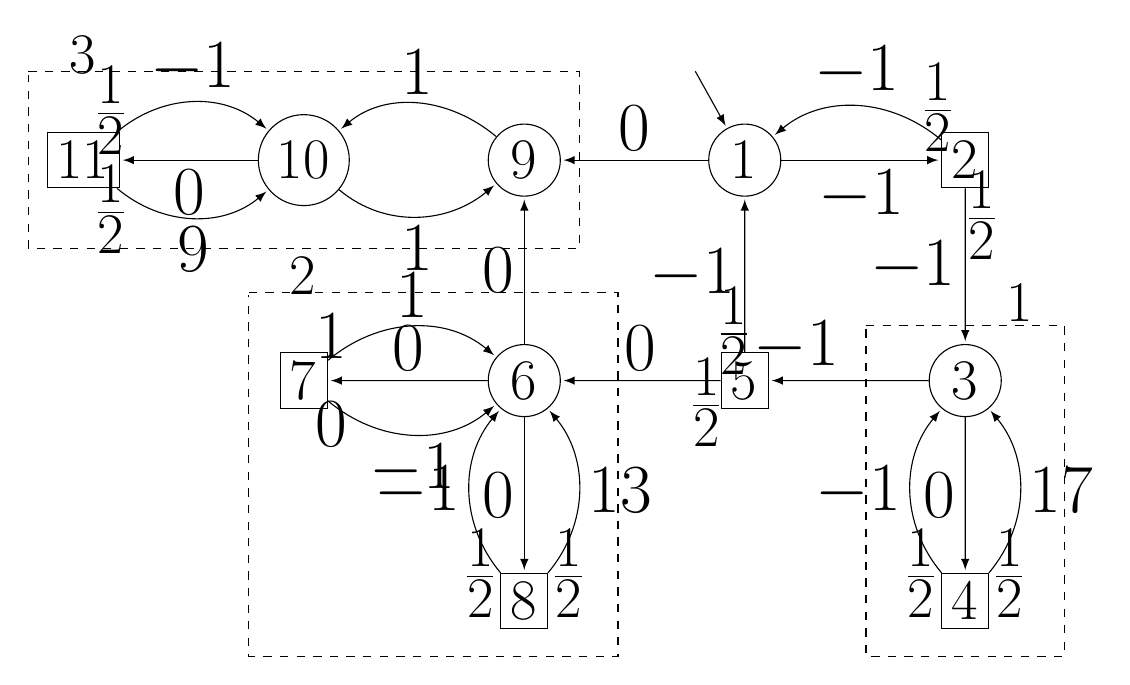
\begin{tikzpicture}[->,>=latex,shorten >=1pt,auto,node
    distance=2.5cm,bend angle=45,font=\Huge,scale=0.7]
    \tikzstyle{p1}=[draw,circle,text centered,minimum size=6mm]
    \tikzstyle{p2}=[draw,rectangle,text centered,minimum size=6mm]
    \tikzstyle{empty}=[]
    \node[p1] (1) at (0,0) {$\state_{9}$};
    \node[p1] (2) at (4,0) {$\state_{1}$};
    \node[p2] (3) at (8,0) {$\state_{2}$};
    \node[p1] (4) at (8,-4) {$\state_{3}$};
    \node[p2] (5) at (8,-8) {$\state_{4}$};
    \node[p2] (6) at (4,-4) {$\state_{5}$};
    \node[p1] (7) at (0,-4) {$\state_{6}$};
    \node[p2] (8) at (-4,-4) {$\state_{7}$};
    \node[p1] (9) at (-4,0) {$\state_{10}$};
    \node[p2] (10) at (-8,0) {$\state_{11}$};
    \node[p2] (11) at (0,-8) {$\state_{8}$};
    \node[empty] (swec) at (-8, 1.9) {$\ec_{3}$};
    \node[empty] (wwec) at (-4, -2.1) {$\ec_{2}$};
    \node[empty] (lec) at (9, -2.6) {$\ec_{1}$};
    \node[empty] (proba5a) at (7.2, -7.5) {$\frac{1}{2}$};
    \node[empty] (proba5b) at (8.8, -7.5) {$\frac{1}{2}$};
    \node[empty] (proba3a) at (8.3, -1) {$\frac{1}{2}$};
    \node[empty] (proba3b) at (7.5, 0.95) {$\frac{1}{2}$};
    \node[empty] (proba8a) at (-3.5, -3.2) {$1$};
    \node[empty] (proba8b) at (-3.5, -4.8) {$0$};
    \node[empty] (proba10a) at (-7.5, 0.9) {$\frac{1}{2}$};
    \node[empty] (proba10b) at (-7.5, -0.9) {$\frac{1}{2}$};
    \node[empty] (proba11a) at (0.8, -7.5) {$\frac{1}{2}$};
    \node[empty] (proba11b) at (-0.8, -7.5) {$\frac{1}{2}$};
    \node[empty] (proba6a) at (3.8, -3.1) {$\frac{1}{2}$};
    \node[empty] (proba6b) at (3.3, -4.4) {$\frac{1}{2}$};
    \coordinate[shift={(-3mm,8mm)}] (init) at (2.north west);
    \path
    (2) edge node[above] {$0$} (1)
    (6) edge node[above] {$0$} (7)
    (4) edge node[above left] {$-1$} (6)
    (3) edge node[left] {$-1$} (4)
    (6) edge node[left] {$-1$} (2)
    (4) edge node[left] {$0$} (5)
    (7) edge node[above] {$0$} (8)
    (7) edge node[left] {$0$} (1)
    (init) edge (2)
    ;
	\draw[->,>=latex] (3) to[out=140,in=40] node[above] {$-1$} (2);
	\draw[->,>=latex] (2) to[out=0,in=180] node[below] {$-1$} (3);
	\draw[->,>=latex] (5) to[out=50,in=310] node[right] {$17$} (4);
	\draw[->,>=latex] (5) to[out=130,in=230] node[left] {$-1$} (4);
	\draw[->,>=latex] (8) to[out=40,in=140] node[above] {$1$} (7);
	\draw[->,>=latex] (8) to[out=320,in=220] node[below] {$-1$} (7);
	\draw[->,>=latex] (1) to[out=140,in=40] node[above] {$1$} (9);
	\draw[->,>=latex] (9) to[out=320,in=220] node[below] {$1$} (1);
	\draw[->,>=latex] (9) to[out=180,in=0] node[below] {$0$} (10);
	\draw[->,>=latex] (10) to[out=40,in=140] node[above] {$-1$} (9);
	\draw[->,>=latex] (10) to[out=320,in=220] node[below] {$9$} (9);
	\draw[->,>=latex] (7) to[out=270,in=90] node[left] {$0$} (11);
	\draw[->,>=latex] (11) to[out=130,in=230] node[left] {$-1$} (7);
	\draw[->,>=latex] (11) to[out=50,in=310] node[right] {$13$} (7);
	\draw[dashed,-] (-9,1.6) -- (1,1.6) -- (1,-1.6) -- (-9,-1.6) -- (-9,1.6);
	\draw[dashed,-] (6.2,-3) -- (9.8,-3) -- (9.8,-9) -- (6.2,-9) -- (6.2,-3);
	\draw[dashed,-] (-5,-2.4) -- (1.7,-2.4) -- (1.7,-9) -- (-5,-9) -- (-5,-2.4);
      \end{tikzpicture}}
      \caption{Beyond worst-case mean-payoff problem: $\ec_{2}$ and $\ec_{3}$ are maximal winning ECs, $\ec_{1}$ is losing.}
\label{12-fig:bwcRunningExample}
  \end{figure}

In order to illustrate several notions and strategies, we will consider the arena depicted in~\cref{12-fig:bwcRunningExample} throughout our presentation. The stochastic model of $\playerTwo$ is memoryless and is described by the probabilities written close to the start of outgoing edges. The colouring (weights) is written besides them.

We consider the $\BWC$ problem with the worst-case threshold $\thresholdWC = 0$. Observe that this arena satisfies the assumptions guaranteed at the end of the preprocessing part of the algorithm. That is, the worst-case threshold is zero, a worst-case winning strategy of $\playerOne$ exists in all vertices (e.g., the memoryless strategy choosing edges $(\state_{1}, \state_{9})$, $(\state_{3}, \state_{5})$, $(\state_{6}, \state_{9})$, $(\state_{9}, \state_{10})$ and $(\state_{10}, \state_{9})$ in their respective starting vertices), and the stochastic model is memoryless, as explained above.
\end{example}


\subsection*{Analysis of end-components} The second part hence operates on an arena $\arena$ such that from all vertices, Eve has a strategy to achieve a strictly positive mean-payoff value (recall that $\alpha = 0$). We consider the MDP $\markovProcess = \arena_{\stratStoch}$ and notice that the underlying graphs of $\arena$ and $\markovProcess$ are the same thanks to $\stratStoch$ being memoryless. The following steps rely on the analysis of "\textit{end-components}" (ECs) in the MDP, i.e., strongly connected subgraphs in which Eve can ensure to stay when playing against Adam's stochastic model (\cref{5-def:ec}).

The motivation to the analysis of ECs is the following. It is well-known that under any arbitrary strategy $\sigma$ of Eve in~$\markovProcess$, the probability that vertices visited infinitely often along a play constitute an EC is one (\cref{5-lem:EC-inf}). Recall that the mean-payoff is prefix independent, therefore the value of any play only depends on those colors that are seen infinitely often. Hence, the expected mean-payoff $\expv^{\sigma}_{\markovProcess,v_0}[\MeanPayoff^{-}]$ depends \textit{uniquely} on the value obtained in the ECs. Inside an EC, we can compute the maximal expected value that can be achieved by Eve, and this value is the same in all vertices of the EC, as established in~\cref{5-thm:mp-valcomp}.

Consequently, in order to satisfy the expected value requirement, an acceptable strategy for the $\BWC$ problem has to favor reaching ECs with a sufficient expectation, but under the constraint that it should also ensure satisfaction of the worst-case requirement. As we show in the following, this constraint implies that some ECs with high expected values may still need to be avoided because they do not permit to guarantee the worst-case requirement. This is the cornerstone of the classification of ECs that follows.

\subsection*{Classification of end-components} Let $\ecsSet \subseteq 2^{V}$ denote the set of all ECs in $\markovProcess$. Notice that by definition, only edges in $\edgesNonZero$, as defined earlier, are involved to determine which sets of vertices form an EC in $\markovProcess$. As such, for any EC $\ec \in \ecsSet$, there may exist edges from $\edges \setminus \edgesNonZero$ starting in $\ec$, such that Adam can force leaving $\ec$ when using an arbitrary strategy in $\arena$. Still these edges will never be used by the stochastic model $\stratStoch$. This remark will be important to the definition of strategies of Eve that guarantee the worst-case requirement, as Eve needs to be able to react to the hypothetical use of such an edge. We will see that it is also the case \textit{inside} an EC.

Now, we want to consider the ECs in which $\playerOne$ can ensure that the worst-case requirement will be fulfilled (i.e., without having to leave the EC): we call them \textit{winning} ECs (WECs). The others will need to be eventually avoided, hence will have zero impact on the expectation of a finite-memory strategy satisfying the $\BWC$ problem. So we call the latter \textit{losing} ECs (LECs). The subtlety of this classification is that it involves considering the ECs both in the MDP~$\markovProcess$, and in the arena~$\arena$.

Formally, let $\ec \in \ecsSet$ be an EC. It is \textit{winning} if, in the subarena induced by $\ec$, from all vertices, $\playerOne$ has a strategy to ensure a \textit{strictly} positive mean-payoff against any strategy of $\playerTwo$ \textit{that only chooses edges which are assigned non-zero probability by $\stratStoch$}, or equivalently, edges in $\edgesNonZero$. This can be interpreted as looking at arena $\gameNonZero$, which is the restriction of $\arena$ to edges in $\edgesNonZero$.

We denote $\winningECs \subseteq \ecsSet$ the set of such ECs. Non-winning ECs are \textit{losing}: in those, whatever the strategy of $\playerOne$ played against the stochastic model $\stratStoch$ (or any strategy with the same support), there exists at least one play for which the mean-payoff is not strictly positive (even if its probability is zero, its mere existence is not acceptable for the worst-case requirement).

\begin{figure}[tbh]
  \centering   
  \scalebox{0.8}{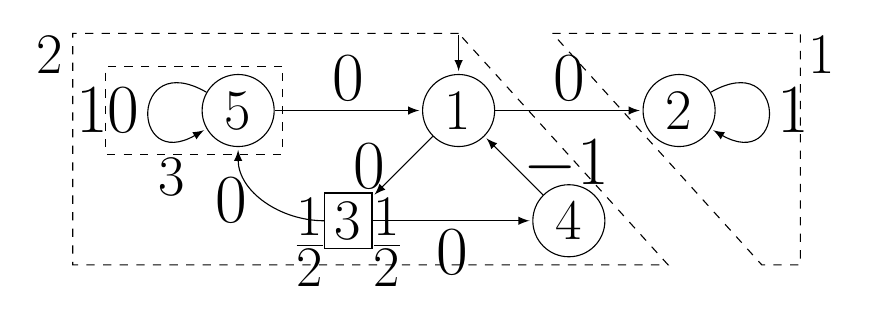
\begin{tikzpicture}[->,>=latex,shorten >=1pt,auto,node
    distance=2.5cm,bend angle=45,font=\Huge,scale=0.7]
    \tikzstyle{p1}=[draw,circle,text centered,minimum size=6mm]
    \tikzstyle{p2}=[draw,rectangle,text centered,minimum size=6mm]
    \tikzstyle{empty}=[]
    \node[p1] (1) at (0,0) {$\state_{1}$};
    \node[p1] (2) at (4,0) {$\state_{2}$};
    \node[p2] (3) at (-2,-2) {$\state_{3}$};
    \node[p1] (4) at (2,-2) {$\state_{4}$};
    \node[p1] (5) at (-4,0) {$\state_{5}$};
    \node[empty] (ec1) at (-5.2, -1.2) {$\ec_{3}$};
    \node[empty] (ec2) at (-7.4, 1) {$\ec_{2}$};
    \node[empty] (ec2) at (6.6, 1) {$\ec_{1}$};
    \node[empty] (proba1) at (-2.7, -2.4) {$\frac{1}{2}$};
    \node[empty] (proba2) at (-1.3, -2.4) {$\frac{1}{2}$};
    \coordinate[shift={(0mm,5mm)}] (init) at (1.north);
    \path
    (1) edge node[above] {$0$} (2)
    (5) edge node[above] {$0$} (1)
    (1) edge node[left,xshift=-1mm] {$0$} (3)
    (4) edge node[right] {$-1$} (1)
    (3) edge node[below] {$0$} (4)
    (init) edge (1)
    (5) edge [loop left, out=150, in=210,looseness=3, distance=16mm] node [left] {$10$} (5)
    (2) edge [loop right, out=30, in=330,looseness=3, distance=16mm] node [right] {$1$} (2)
    ;
	\draw[->,>=latex] (3) to[out=180,in=270] node[left,xshift=-1mm] {$0$} (5);
	\draw[dashed,-] (-3.2,0.8) -- (-6.4,0.8) -- (-6.4,-0.8) -- (-3.2,-0.8) -- (-3.2,0.8);
	\draw[dashed,-] (0,1.4) -- (-7,1.4) -- (-7,-2.8) -- (3.8,-2.8) -- (0,1.4);
	\draw[dashed,-] (1.7,1.4) -- (6.2,1.4) -- (6.2,-2.8) -- (5.5,-2.8) -- (1.7,1.4);
      \end{tikzpicture}}
      \caption{EC $\ec_{2}$ is losing. The set of MWECs is $\maxWinningECs = \winningECs = \{\ec_{1}, \ec_{3}\}$.}
\label{12-fig:bwcWinningECsComputationExample}
  \end{figure}

\begin{example}
Note that an EC is winning if $\playerOne$ has a worst-case winning strategy from \textit{all} vertices. This point is important as it may well be the case that winning strategies exist in a strict subset of vertices of the EC. This does not contradict the definition of ECs as strongly connected subgraphs, as the latter only guarantees that every vertex can be reached \textit{with probability one}, and not necessarily \textit{surely}. Hence one cannot call upon the prefix independence of the mean-payoff to extend the existence of a winning strategy to all vertices.

Such a situation can be observed on the arena of~\cref{12-fig:bwcWinningECsComputationExample}, where the EC~$\ec_{2}$ is losing (because from $\state_{1}$, the play $(\state_{1}\state_{3}\state_{4})^{\omega}$ can be forced by $\playerTwo$, yielding mean-payoff $-1/3 \leq 0$), while its sub-EC~$\ec_{3}$ is winning. From $\state_{1}$, $\playerOne$ can ensure to reach $\ec_{3}$ "almost-surely", but not "surely", which is critical in this case.
\end{example}


\subsection*{Maximal winning end-components} Based on these definitions, observe that~\cref{12-algo:BWC} does not actually compute the set $\winningECs$ containing all WECs, but rather the set $\maxWinningECs \subseteq \winningECs$, defined as $\maxWinningECs = \{\ec \in \winningECs \mid \forall\, \ec' \in \winningECs,\, \ec \subseteq \ec' \Rightarrow \ec = \ec'\}$, i.e., the set of \textit{maximal} WECs (MWECs).

The intuition on \textit{why we can} restrict our study to this subset is as follows. If an EC $\ec_{1} \in \winningECs$ is included in another EC $\ec_{2} \in \winningECs$, i.e., $\ec_{1} \subseteq \ec_{2}$, we have that the maximal expected value achievable in $\ec_{2}$ is at least equal to the one achievable in~$\ec_{1}$. Indeed, $\playerOne$ can reach $\ec_{1}$ with probability one (by virtue of $\ec_{2}$ being an EC and $\ec_{1} \subseteq \ec_{2}$) and stay in it forever with probability one (by virtue of $\ec_{1}$ being an EC): hence the expectation of such a strategy would be equal to what can be obtained in~$\ec_{1}$ thanks to the prefix independence of the mean-payoff. This property implies that it is sufficient to consider MWECs in our computations.

As for \textit{why we do it}, observe that the complexity gain is critical. The number of WECs can be as large as~$\vert\winningECs\vert \leq \vert\ecsSet\vert \leq 2^{\vert V\vert}$, that is, exponential in the size of the input. Yet, the number of MWECs is bounded by $\vert\maxWinningECs\vert \leq \vert V\vert$ as they are disjoint by definition: for any two WECs with a non-empty intersection, their union also constitutes an EC, and is still winning because $\playerOne$ can essentially stick to the EC of her choice.

The computation of the set $\maxWinningECs$ is executed by a recursive subalgorithm calling polynomially-many times an oracle solving the worst-case problem (e.g., following the pseudo-polynomial-time algorithm of~\cref{chap:payoffs}). \todo{I need a label on Subsect. 4.3.4 to cite it precisely.} Roughly sketched, this algorithm computes the maximal EC decomposition of an MDP (in polynomial time by~\cref{5-thm:MEC-decomposition-complexity}), then checks for each EC $\ec$ in the decomposition (their number is polynomial) if $\ec$ is winning or not, which requires a call to an oracle solving the worst-case threshold problem on the corresponding subgame. If $\ec$ is losing, it may still be the case that a sub-EC $\ec' \subsetneq \ec$ is winning. Therefore we recurse on the MDP reduced to $\ec$, where vertices from which $\playerTwo$ can win in $\ec$ have been removed (they are a no-go for $\playerOne$). Hence the stack of calls is also at most polynomial.

\begin{lemma}
\label{12-lem:MWEC}
The set $\maxWinningECs$ of MWECs can be computed in pseudo-polynomial time, and deciding if a set of vertices $U \subseteq V$ belongs to $\maxWinningECs$ is in $\NP \cap \coNP$.
\end{lemma}

The complexity follows from~\cref{4-thm:MP-NPcoNP} and $\P^{\NP \cap \coNP} = \NP \cap \coNP$~\cite{Brassard:1979}.

\begin{example}
Consider the running example in~\cref{12-fig:bwcRunningExample}. Note that vertices $\state_{1}$, $\state_{2}$ and $\state_{5}$ do not belong to any EC: given any strategy of $\playerOne$ in $\markovProcess$, with probability one, any consistent play will only visit these vertices a finite number of times (\cref{5-lem:EC-inf}). The set of \textit{MWECs} is $\maxWinningECs = \{\ec_{2}, \ec_{3}\}$. Obviously, these ECs are disjoint. The set of WECs is larger, $\winningECs = \maxWinningECs \cup \{\{\state_{9}, \state_{10}\}, \{\state_{6}, \state_{7}\}\}$.

End-component $\ec_{1}$ is \textit{losing}: in the subarena $\gameNonZero \reduc \ec_{1}$, Adam's strategy consisting in always picking the $-1$ edge guarantees a negative mean-payoff. Note that this edge is present in $\edgesNonZero$ as it is assigned probability $1/2$ by the stochastic model $\stratStoch$. Here, we witness why it is important to base our definition of WECs on $\gameNonZero$ rather than $\arena$. Indeed, in $\arena \reduc \ec_{2}$, it is also possible for $\playerTwo$ to guarantee a negative mean-payoff by always choosing edges with weight $-1$. However, to achieve this, $\playerTwo$ has to pick edges that are \textit{not} in $\edgesNonZero$: this will never happen against the stochastic model and as such, this can be watched by $\playerOne$ to see if $\playerTwo$ uses an arbitrary antagonistic strategy, and dealt with. If $\playerTwo$ conforms to $\edgesNonZero$, i.e., if he plays in $\gameNonZero$, he has to pick the edge of weight $1$ in $\state_{7}$ and $\playerOne$ has a worst-case winning strategy consisting in always choosing to go in $\state_{7}$. This EC is thus classified as \textit{winning}. Note that for $\ec_{3}$, in both subarenas $\arena \reduc \ec_{3}$ and $\gameNonZero \reduc \ec_{3}$, $\playerOne$ can guarantee a strictly positive mean-payoff by playing $(\state_{9}\,\state_{10})^\omega$: even \textit{arbitrary} strategies of $\playerTwo$ cannot endanger $\playerOne$ in this case.

Lastly, consider the arena depicted in~\cref{12-fig:bwcWinningECsComputationExample}. While $\ec_{2}$ is a strict superset of $\ec_{3}$, the former is losing whereas the latter is winning, as explained above. Hence, the set $\maxWinningECs$ is equal to $\{\ec_{1}, \ec_{3}\}$.
\end{example}

\subsection*{Ensure reaching winning end-components} As discussed, under any arbitrary strategy of $\playerOne$, vertices visited infinitely often form an EC with probability one (\cref{5-lem:EC-inf}). Now, if we take a \textit{finite-memory} strategy that \textit{satisfies} the $\BWC$ problem, we can refine this result and state that they form a \textit{winning} EC with probability one. Equivalently, let $\infVisited{\play}$ denote the set of vertices visited infinitely often along a play $\play$: we have that the probability that a play~$\play$ is such that $\infVisited{\play} = \ec$ for some $\ec \in \ecsSet \setminus \winningECs$ is zero. The equality is crucial. It may be the case, with non-zero probability, that $\infVisited{\play} = \ec' \subsetneq \ec$, for some $\ec' \in \winningECs$, and $\ec \in \ecsSet \setminus \winningECs$ (hence the recursive algorithm to compute $\maxWinningECs$). It is clear that~$\playerOne$ should not visit all the vertices of a LEC forever, as then she would not be able to guarantee the worst-case threshold inside the corresponding subarena.\footnote{This is no longer true if Eve may use infinite memory: there may still be some incentive to stay in a LEC. But this goes beyond the scope of our overview.}

\begin{lemma}
\label{12-lem:EC-inf}
For any initial vertex $ v_0 $ and finite-memory strategy $ \sigma $ that satisfies the BWC problem, it holds that $ \probm^\sigma_{\markovProcess, v_0} ( \{\play \mid \infVisited{\play} \in \winningECs \}) = 1 $. 
\end{lemma}

We denote $\negligibleStates = V \setminus \bigcup_{\ec \in \maxWinningECs} \ec$ the set of vertices that, with probability one, are only seen a finite number of times when a $\BWC$ satisfying strategy is played, and call them \textit{negligible} vertices.

Our ultimate goal here is to modify the colouring of $\markovProcess$ from $c$ to $c'$, such that a classical optimal strategy for the expected value problem (\cref{5-thm:general-mp-main}) using this new colouring $c'$ will naturally avoid LECs and prescribe which WECs are the most interesting to reach for a $\BWC$ strategy on the initial arena $\arena$ and MDP $\markovProcess$ with colouring $c$. For the sake of readability, let us simply use $\markovProcess$ and $\markovProcess'$ to refer to MDP $\markovProcess$ with respective colourings $c$ and $c'$.

Observe that the expected value obtained in $\markovProcess$ by any $\BWC$ satisfying strategy of $\playerOne$ only depends on the weights of edges involved in WECs, or equivalently, in MWECs (as the set of plays that are not trapped in them has measure zero). Consequently, we define colouring $c'$ as follows: we keep the weights unchanged in edges that belong to some $\ec \in \maxWinningECs$, and we put them to zero everywhere else, i.e., on any edge involving a negligible vertex. Weight zero is taken because it is lower than the expectation granted by WECs, which is \textit{strictly} greater than zero by definition (as $\alpha = 0$).

\begin{example}
Consider $\ec_{1}$ in~\cref{12-fig:bwcRunningExample}. This EC is losing as argued before. The optimal expectation achievable in $\markovProcess \reduc \ec_{1}$ by $\playerOne$ is $4$: this is higher than what is achievable in both $\ec_{2}$ and $\ec_{3}$. Note that there exists no WEC included in $\ec_{1}$. By~\cref{chap:mdp}, we know that any strategy of $\playerOne$ will see its expectation bounded by the maximum between the optimal expectations of the ECs $\ec_{1}$, $\ec_{2}$ and $\ec_{3}$. Our previous arguments further refine this bound by restricting it to the maximum between the expectations of $\ec_{2}$ and $\ec_{3}$. Indeed, $\playerOne$ cannot benefit from the expected value of $\ec_{1}$ while using finite memory, as being trapped in~$\ec_{1}$ induces the existence of plays losing for the worst-case. Hence there is no point in playing inside $\ec_{1}$ and $\playerOne$ may as well cross it directly and try to maximize its expectation using the WECs, $\ec_{2}$ and $\ec_{3}$. The set of negligible vertices in $\markovProcess$ is $\negligibleStates = V \setminus (\ec_{2} \cup \ec_{3}) = \{\state_{1}, \state_{2}, \state_{3}, \state_{4}, \state_{5}\}$. We depict $\markovProcess'$ in~\cref{12-fig:bwc_mp_modifiedMDP}.

In the arena depicted in~\cref{12-fig:bwcWinningECsComputationExample}, we already observed that $\ecsSet = \{\ec_{1}, \ec_{2}, \ec_{3}\}$ and $\winningECs = \maxWinningECs = \{\ec_{1}, \ec_{3}\}$. Consider the negligible vertex $\state_{1} \in \negligibleStates = \ec_{2} \setminus \ec_{3}$. A finite-memory strategy of $\playerOne$ may only take the edge $(\state_{1}, \state_{3})$ finitely often in order to ensure the worst-case requirement. If $\playerOne$ were to play this edge repeatedly, the losing play $(\state_{1}\state_{3}\state_{4})^{\omega}$ would exist (while of probability zero). Therefore, $\playerOne$ can only ensure that $\ec_{3}$ is reached with a probability arbitrarily close to one, and not equal to one, because at some point, she has to switch to edge $(\state_{1}, \state_{2})$ (after a bounded time since $\playerOne$ uses a finite-memory strategy).
\end{example}

\begin{figure}[htb]
  \centering   
  \scalebox{0.8}{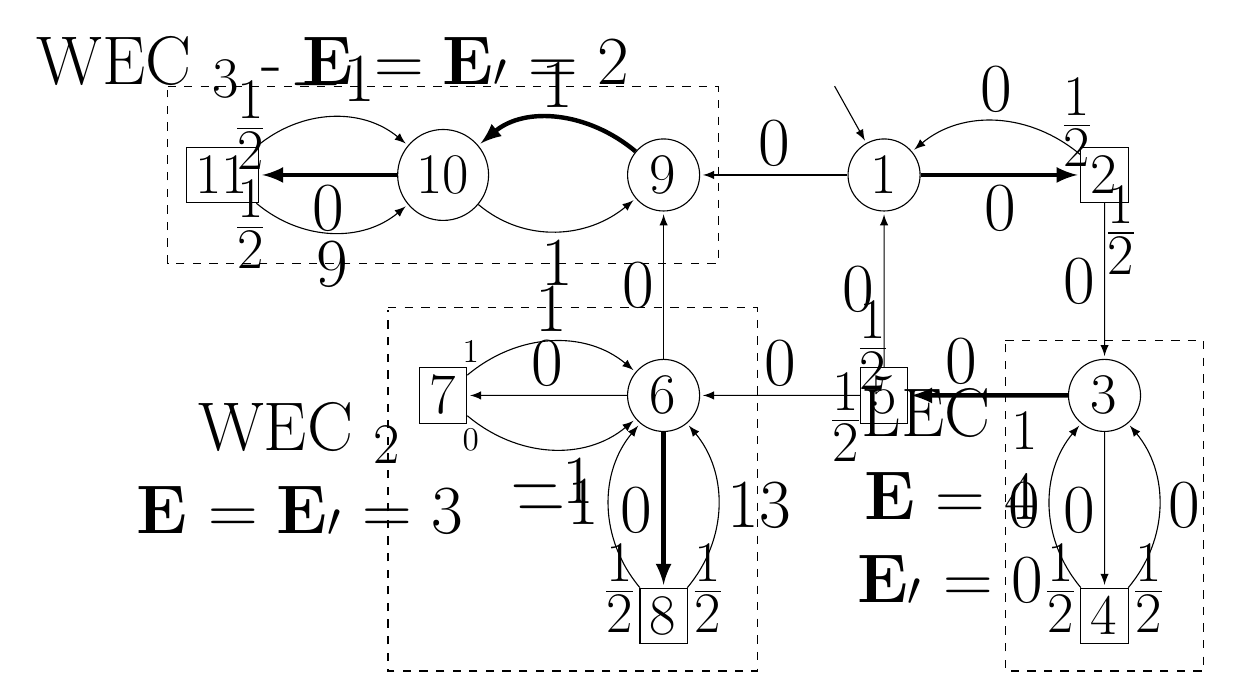
\begin{tikzpicture}[->,>=latex,shorten >=1pt,auto,node
    distance=2.5cm,bend angle=45,font=\Huge,scale=0.7]
    \tikzstyle{p1}=[draw,circle,text centered,minimum size=6mm]
    \tikzstyle{p2}=[draw,rectangle,text centered,minimum size=6mm]
    \tikzstyle{empty}=[]
    \node[p1] (1) at (0,0) {$\state_{9}$};
    \node[p1] (2) at (4,0) {$\state_{1}$};
    \node[p2] (3) at (8,0) {$\state_{2}$};
    \node[p1] (4) at (8,-4) {$\state_{3}$};
    \node[p2] (5) at (8,-8) {$\state_{4}$};
    \node[p2] (6) at (4,-4) {$\state_{5}$};
    \node[p1] (7) at (0,-4) {$\state_{6}$};
    \node[p2] (8) at (-4,-4) {$\state_{7}$};
    \node[p1] (9) at (-4,0) {$\state_{10}$};
    \node[p2] (10) at (-8,0) {$\state_{11}$};
    \node[p2] (11) at (0,-8) {$\state_{8}$};
    \node[empty] (swec) at (-6, 1.9) {WEC $\ec_{3}$ - $\expv_{\markovProcess} = \expv_{\markovProcess'} = 2$};
    \node[empty,align=center] (wwec) at (-6.6, -5.5) {WEC $\ec_{2}$\\$\expv_{\markovProcess} = \expv_{\markovProcess'} = 3$};
    \node[empty,align=center] (lec) at (5.2, -6) {LEC $\ec_{1}$\\$\expv_{\markovProcess} = 4$\\$\expv_{\markovProcess'}  = 0$};
    \node[empty] (proba5a) at (7.2, -7.5) {$\frac{1}{2}$};
    \node[empty] (proba5b) at (8.8, -7.5) {$\frac{1}{2}$};
    \node[empty] (proba3a) at (8.3, -1) {$\frac{1}{2}$};
    \node[empty] (proba3b) at (7.5, 0.95) {$\frac{1}{2}$};
    \node[empty] (proba8a) at (-3.5, -3.2) {{\large $1$}};
    \node[empty] (proba8b) at (-3.5, -4.8) {{\large $0$}};
    \node[empty] (proba10a) at (-7.5, 0.9) {$\frac{1}{2}$};
    \node[empty] (proba10b) at (-7.5, -0.9) {$\frac{1}{2}$};
    \node[empty] (proba11a) at (0.8, -7.5) {$\frac{1}{2}$};
    \node[empty] (proba11b) at (-0.8, -7.5) {$\frac{1}{2}$};
    \node[empty] (proba6a) at (3.8, -3.1) {$\frac{1}{2}$};
    \node[empty] (proba6b) at (3.3, -4.4) {$\frac{1}{2}$};
    \coordinate[shift={(-3mm,8mm)}] (init) at (2.north west);
    \path
    (2) edge node[above] {$0$} (1)
    (6) edge node[above] {$0$} (7)
    (4) edge[ultra thick] node[above left] {$0$} (6)
    (3) edge node[left] {$0$} (4)
    (6) edge node[left] {$0$} (2)
    (4) edge node[left] {$0$} (5)
    (7) edge node[above] {$0$} (8)
    (7) edge node[left] {$0$} (1)
    (init) edge (2)
    ;
	\draw[->,>=latex] (3) to[out=140,in=40] node[above] {$0$} (2);
	\draw[->,>=latex,ultra thick] (2) to[out=0,in=180] node[below] {$0$} (3);
	\draw[->,>=latex] (5) to[out=50,in=310] node[right] {$0$} (4);
	\draw[->,>=latex] (5) to[out=130,in=230] node[left] {$0$} (4);
	\draw[->,>=latex] (8) to[out=40,in=140] node[above] {$1$} (7);
	\draw[->,>=latex] (8) to[out=320,in=220] node[below] {$-1$} (7);
	\draw[->,>=latex,ultra thick] (1) to[out=140,in=40] node[above] {$1$} (9);
	\draw[->,>=latex] (9) to[out=320,in=220] node[below] {$1$} (1);
	\draw[->,>=latex,ultra thick] (9) to[out=180,in=0] node[below] {$0$} (10);
	\draw[->,>=latex] (10) to[out=40,in=140] node[above] {$-1$} (9);
	\draw[->,>=latex] (10) to[out=320,in=220] node[below] {$9$} (9);
	\draw[->,>=latex,ultra thick] (7) to[out=270,in=90] node[left] {$0$} (11);
	\draw[->,>=latex] (11) to[out=130,in=230] node[left] {$-1$} (7);
	\draw[->,>=latex] (11) to[out=50,in=310] node[right] {$13$} (7);
	\draw[dashed,-] (-9,1.6) -- (1,1.6) -- (1,-1.6) -- (-9,-1.6) -- (-9,1.6);
	\draw[dashed,-] (6.2,-3) -- (9.8,-3) -- (9.8,-9) -- (6.2,-9) -- (6.2,-3);
	\draw[dashed,-] (-5,-2.4) -- (1.7,-2.4) -- (1.7,-9) -- (-5,-9) -- (-5,-2.4);
      \end{tikzpicture}}
      \caption{Putting all weights outside MWECs to zero naturally drives the optimal expectation strategy in $\markovProcess'$, depicted by the thick edges, toward the highest valued MWECs. ECs are annotated with their corresponding optimal expectations in the original MDP $\markovProcess$ and the modified MDP $\markovProcess'$.}
\label{12-fig:bwc_mp_modifiedMDP}
  \end{figure}

\subsection*{Reach the highest valued winning end-components} We compute the maximal expected mean-payoff $\beta^{\ast}$ that can be achieved by $\playerOne$ in $\markovProcess'$, from $v_0$. This computation takes polynomial time and memoryless strategies suffice to achieve the maximal value, as established in~\cref{5-thm:general-mp-main}.

As discussed before, such a strategy reaches an EC of $\markovProcess'$ with probability one. Basically, we build a strategy that favours reaching ECs with high associated expectations in $\markovProcess'$.

We argue that the ECs reached with probability one by this strategy are necessarily WECs in $\markovProcess$. Clearly, if a WEC is reachable instead of a losing one, it will be favoured because of the weights definition in $\markovProcess'$ (expectation is strictly higher in WECs). Thus it remains to check if the set of WECs is reachable with probability one from any vertex in $V$. That is the case because of the preprocessing: we know that all vertices are winning for the worst-case requirement. Clearly, from any vertex in $A = V \setminus \bigcup_{\ec \in \ecsSet} \ec$, $\playerOne$ cannot ensure to stay in $A$ (otherwise it would form an EC) and thus must be able to win the worst-case requirement from reached ECs. Now for any vertex in $B = \bigcup_{\ec \in \ecsSet} \ec \setminus \bigcup_{\ec \in \maxWinningECs} \ec$, i.e., vertices in LECs and not in any sub-EC winning, $\playerOne$ cannot win the worst-case by staying in $B$, by definition of LEC. Since we know $\playerOne$ can ensure the worst-case by hypothesis, it is clear that she must be able to reach $C = \bigcup_{\ec \in \maxWinningECs} \ec$ from any vertex in $B$, as claimed.

\subsection*{Inside winning end-components} Based on that, we know that WECs of $\markovProcess$ will be reached with probability one when maximizing the expected value in $\markovProcess'$. Let us first consider what we can say about such ECs if we assume that $\edgesNonZero = \edges$, i.e., if the stochastic model $\stratStoch$ maps all possible edges to non-zero probabilities. 
We establish a finite-memory \textit{combined strategy} $\stratComb$ of $\playerOne$ that ensures~(i) worst-case satisfaction while yielding (ii) an expected value $\varepsilon$-close to the maximal expectation inside the EC.

For two well-chosen parameters $\stepsExp, \stepsWC \in \N$, it is informally defined as follows: in phase $\typeA$, play a memoryless expected value optimal strategy $\stratExp$ for $\stepsExp$ steps and memorize $\cmbSum \in \Z$, the sum of weights along these steps; in phase $\typeB$, if $\cmbSum > 0$, go to~$\typeA$, otherwise play a memoryless worst-case optimal strategy $\stratWC$ for~$\stepsWC$ steps, then go to $\typeA$. In $\typeA$, $\playerOne$ tries to increase her expectation and approach the optimal one, while in $\typeB$, she compensates, if needed, losses that occurred in $\typeA$.

The two memoryless strategies exist on the subarena induced by the EC: by definition of ECs, based on~$\edgesNonZero$, the stochastic model of $\playerTwo$ will never be able to force leaving the EC against the combined strategy.

A key result to our approach is the existence of values for $\stepsExp$ and~$\stepsWC$ such that~(i) and (ii) are verified. We see plays as sequences of periods, each starting with phase~$\typeA$.

First, for any $\stepsExp$, it is possible to define $\stepsWC(\stepsExp)$ such that any period composed of phases~$\typeA+\typeB$ ensures a mean-payoff at least $1/(\stepsExp+\stepsWC) > 0$. Periods containing only phase $\typeA$ trivially induce a mean-payoff at least~$1/\stepsExp$ as they are not followed by phase $\typeB$. Both rely on the weights being integers. As the length of any period is bounded by $(\stepsExp+\stepsWC)$, the inequality remains strict for the mean-payoff of any play, granting~(i).

Now, consider parameter $\stepsExp$. Clearly, when~$\stepsExp \rightarrow \infty$, the expectation over phase $\typeA$ tends to the optimal one. Nevertheless, phases~$\typeB$ also contribute to the overall expectation of the combined strategy, and (in general) lower it so that it is strictly less than the optimal for any $\stepsExp, \stepsWC \in \N$. Hence to prove (ii), we not only need that the probability of playing phase $\typeB$ decreases when $\stepsExp$ increases, but also that it decreases faster than the increase of $\stepsWC$, needed to ensure~(i), so that overall, the contribution of phases~$\typeB$ tends to zero when $\stepsExp \rightarrow \infty$. This is indeed the case and is proved using results bounding the probability of observing a mean-payoff significantly (more than some $\varepsilon$) different than the optimal expectation along a phase $\typeA$ of length $\stepsExp \in \N$: this probability decreases exponentially when~$\stepsExp$ increases, while $\stepsWC$ only needs to be polynomial in $\stepsExp$.

\begin{theorem}
\label{12-thm:insideWinning}
Let $U \in \winningECs$ be a WEC, $\stratStoch$ be such that $\edgesNonZero = \edges$, $v_0 \in U$ be the initial vertex, and let $\beta^\ast \in \Q$ be the maximal expected value achievable by $\playerOne$ in EC $U$. Then, for all~$\varepsilon > 0$, there exists a finite-memory strategy of $\playerOne$ that satisfies the $\BWC$ problem for the thresholds pair $(0,\, \beta^\ast - \varepsilon)$.
\end{theorem}

\begin{example}
Consider the subarena $\gameNonZero \reduc \ec_{3} = \arena \reduc \ec_{3}$ from~\cref{12-fig:bwcRunningExample} and the initial vertex $\state_{10}$. Clearly, the worst-case requirement can be satisfied, that is why the EC is classified as winning. Always choosing to go to~$\state_{9}$ when in $\state_{10}$ is an optimal memoryless worst-case strategy $\stratWC$ that guarantees a mean-payoff $\alpha^\ast = 1$. Its expectation is $\expv^{\stratWC}_{(\arena \reduc \ec_{3})_{\tau^\text{stoch}},v_{10}}[\MeanPayoff^{-}] = 1$. On the other hand, the strategy $\stratExp$ that always selects the edge going to $\state_{11}$ is optimal regarding the expected value criterion: it induces expectation $\beta^\ast = \big(0 + \big(1/2 \cdot 9 + 1/2 \cdot (-1)\big)\big)/2 = 2$ against the stochastic model $\stratStoch$. However, it can only guarantee a mean-payoff of value $-1/2$ in the worst-case.

By the reasoning above, we know that it is possible to find finite-memory strategies satisfying the $\BWC$ problem for any thresholds pair $(0,\, 2 - \varepsilon)$, $\varepsilon > 0$. In particular, consider the thresholds pair $(0,\, 3/2)$. We build a combined strategy~$\stratComb$ as sketched before. Let $\stepsExp = \stepsWC = 2$: the strategy plays the edge $(\state_{10}, \state_{11})$ once, then if the edge of value $9$ has been chosen by $\playerTwo$, it chooses $(\state_{10}, \state_{11})$ again; otherwise it chooses the edge $(\state_{10}, \state_{9})$ once and then resumes choosing $(\state_{10}, \state_{11})$. This strategy satisfies the $\BWC$ problem. In the worst-case,~$\playerTwo$ always chooses the $-1$ edge, but each time he does so, the $-1$ is followed by two~$+1$ thanks to the cycle $\state_{10} \state_{9} \state_{10}$. Strategy $\stratComb$ hence guarantees a mean-payoff equal to $(0 - 1 + 1 + 1)/4 = 1/4 > 0$ in the worst-case. For the expected value requirement, we can build the induced Markov chain $(\arena \reduc \ec_{3})_{\stratComb, \tau^\text{stoch}}$ (\cref{12-fig:mp_insideSWEC_MC}) and check that its expectation is $\expv^{\stratComb}_{(\arena \reduc \ec_{3})_{\tau^\text{stoch}},v_{10}}[\MeanPayoff^{-}] = 5/3 > 3/2$ (\cref{chap:payoffs}).

\begin{figure}[ht]
  \centering 
  \scalebox{0.8}{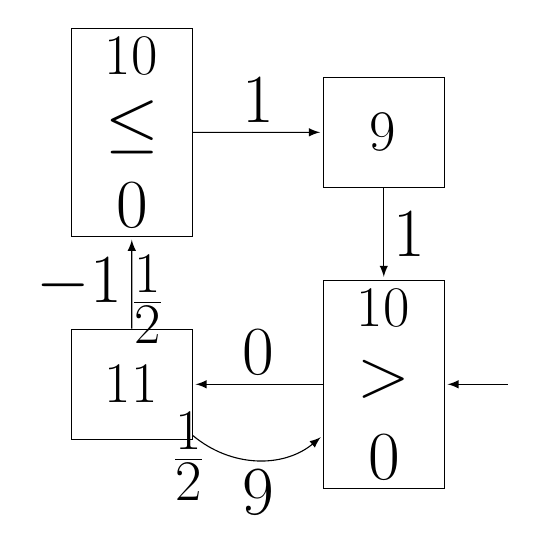
\begin{tikzpicture}[->,>=latex,shorten >=1pt,auto,node
    distance=2.5cm,bend angle=45,font=\Huge,scale=0.8]
    \tikzstyle{p1}=[draw,circle,text centered,minimum size=6mm]
    \tikzstyle{p2}=[draw,rectangle,text centered,minimum size=14mm,text width=13mm]
    \tikzstyle{p3}=[draw,diamond,text centered,minimum size=20mm,text width=13mm]
    \tikzstyle{empty}=[]
    \node[p2] (1) at (0,0) {$\state_{10}$\\$\cmbSum > 0$};
    \node[p2] (2) at (-4,0) {$\state_{11}$};
    \node[p2] (3) at (-4,4) {$\state_{10}$\\$\cmbSum \leq 0$};
    \node[p2] (4) at (0,4) {$\state_{9}$};
    \node[empty] (a) at (-3.75, 1.35) {$\frac{1}{2}$};
    \node[empty] (b) at (-3.10, -1.15) {$\frac{1}{2}$};
    \coordinate[shift={(8mm,0mm)}] (init) at (1.east);
    \path
    (1) edge node[above] {$0$} (2)
    (2) edge node[left] {$-1$} (3)
    (3) edge node[above] {$1$} (4)
    (4) edge node[right] {$1$} (1)
    (init) edge (1)
    ;
	\draw[->,>=latex] (2) to[out=320,in=220] node[below] {$9$} (1);
      \end{tikzpicture}}
      \caption{Markov chain induced by the combined strategy $\stratComb$ and the stochastic model $\stratStoch$ over the WEC $\ec_{3}$ of $\arena$.}
\label{12-fig:mp_insideSWEC_MC}
\end{figure}
\end{example}

\begin{remark}
\label{12-rmk:bwcMemorylessNotEnough}
Memoryless strategies do not suffice for the $\BWC$ problem, even with randomization. Indeed, the edge $(\state_{10}, \state_{11})$ cannot be assigned a non-zero probability as it would endanger the worst-case requirement (since the play~$(\state_{10}\state_{11})^{\omega}$ cycling on the edge of weight $-1$ would exist and have a negative mean-payoff). Hence, the only acceptable memoryless strategy is $\stratWC$, which has only an expectation of $1$.
\end{remark}


Now, consider what happens if $\edgesNonZero \subsetneq E$. Then, if $\playerTwo$ uses an arbitrary strategy, he can take edges of probability zero, i.e., in $E \setminus \edgesNonZero$, either staying in the EC, or leaving it. In both cases, this must be taken into account in order to satisfy the worst-case constraint as it may involve dangerous weights (recall that zero-probability edges are not considered when an EC is classified as winning or not). Fortunately, if this were to occur, $\playerOne$ could switch to a worst-case winning memoryless strategy $\stratSecure$, which exists in all vertices thanks to the preprocessing, to preserve the worst-case requirement. Regarding the expected value, this has no impact as it occurs with probability zero against $\stratStoch$. The strategy to follow in WECs hence adds this reaction procedure to the combined strategy: we call it the \textit{witness-and-secure strategy} $\stratWNS$.

\begin{theorem}
\label{12-thm:wns}
Let $U \in \winningECs$ be a WEC, $v_0 \in U$ be the initial vertex, and $\beta^\ast \in \Q$ be the maximal expected value achievable by $\playerOne$ in EC $U$. Then, for all~$\varepsilon > 0$, there exists a finite-memory strategy of $\playerOne$ that satisfies the $\BWC$ problem for the thresholds pair $(0,\, \beta^\ast - \varepsilon)$.
\end{theorem}

\begin{example}
Consider the WEC $\ec_{2}$ in~\cref{12-fig:bwcRunningExample} and the initial vertex $\state_{6} \in \ec_{2}$. $\playerOne$ can ensure a strictly positive mean-payoff in the subarena $\gameNonZero \reduc \ec_{2}$, but not in $\arena \reduc \ec_{2}$. Indeed, it is easy to see that by always choosing the $-1$ edges (which requires an edge $(\state_{7}, \state_{6}) \in \edgesNonZero \setminus \edges$), $\playerTwo$ can ensure a negative mean-payoff whatever the strategy of $\playerOne$. However, there exists a strategy that ensures the worst-case constraint, i.e., that yields a strictly positive mean-payoff against any strategy of Adam, by leaving the EC. Let $\stratSecure$ be the memoryless strategy that takes the edge $(\state_{6}, \state_{9})$ and then cycle on $(\state_{10}\state_{9})^{\omega}$ forever: it guarantees a mean-payoff of $1 > 0$.

For a moment, consider the EC $\ec_{2}$ in $\gameNonZero$. Graphically, it means that the $-1$ edge from $\state_{7}$ to $\state_{6}$ disappears. In the subarena $\gameNonZero \reduc \ec_{2}$, there are two particular memoryless strategies. The optimal worst-case strategy $\stratWC$ guarantees a mean-payoff of $1/2 > 0$ by choosing to go to $\state_{7}$. The optimal expectation strategy $\stratExp$ yields an expected mean-payoff of $3$ by choosing to go to $\state_{8}$ (naturally this strategy yields the same expectation whether we consider edges in $\edgesNonZero$ or in $E$). Based on them, we build the combined strategy $\stratComb$ of Eve as defined earlier and by~\cref{12-thm:insideWinning}, for any $\varepsilon > 0$, there are values of $\stepsExp$ and $\stepsWC$ such that it satisfies the $\BWC$ problem for thresholds $(0,\, 3-\varepsilon)$ in $\gameNonZero \reduc \ec_{2}$. For instance, for $\stepsExp = \stepsWC = 2$, we have $\expv^{\stratComb}_{(\arena \reduc \ec_{2})_{\tau^\text{stoch}},v_{6}}[\MeanPayoff^{-}] = 13/6$.

We construct the witness-and-secure strategy $\stratWNS$ based on $\stratComb$ and $\stratSecure$ as described above. In this case, that means playing as $\stratComb$ until the $-1$ edge from $\state_{7}$ to $\state_{6}$ is taken by $\playerTwo$. This strategy ensures a worst-case mean-payoff equal to $1 > 0$ thanks to $\stratSecure$ and yields expectation $\expv^{\stratWNS}_{(\arena \reduc \ec_{2})_{\tau^\text{stoch}},v_{6}}[\MeanPayoff^{-}] = 13/6$ for $\stepsExp = \stepsWC = 2$.

Finally, notice that securing the mean-payoff by switching to  $\stratSecure$ \textit{is needed} to satisfy the worst-case requirement if $\playerTwo$ plays in $\edges \setminus \edgesNonZero$. Also, observe that it is still necessary to alternate according to $\stratComb$ in $\gameNonZero \reduc \ec_{2}$ and that playing $\stratExp$ is not sufficient to ensure the worst-case (because $\playerOne$ has to deal with the $-1$ edge from $\state_{8}$ to $\state_{6}$ that remains in $\edgesNonZero$).
\end{example}


\subsection*{Global strategy synthesis} In summary, (a) LECs should be avoided and will be by a strategy that optimizes the expectation on the MDP~$\markovProcess'$; (b) in WECs, $\playerOne$ can obtain ($\varepsilon$-closely) the expectation of the EC \textit{and} ensure the worst-case threshold.

Hence, we finally compare the value $\thresholdExp^{\ast}$ computed by~\cref{12-algo:BWC} with the expected value threshold $\thresholdExp$: (i) if it is strictly higher, we conclude that there exists a finite-memory strategy satisfying the $\BWC$ problem, and (ii) if it is not, we conclude that there does not exist such a strategy.

To prove (i), we establish a finite-memory strategy in $\arena$, called \textit{global strategy} $\stratGlobal$, of $\playerOne$ that ensures a strictly positive mean-payoff against an antagonistic adversary, and ensures an expected mean-payoff $\varepsilon$-close to $\thresholdExp^{\ast}$ (hence, strictly greater than $\thresholdExp$) against the stochastic adversary modeled by $\stratStoch$ (i.e., in $\markovProcess$). The intuition is as follows. We play the memoryless optimal strategy of $\markovProcess'$ for a sufficiently long time, defined by a parameter $\stepsGlobal \in \N$, in order to be with probability close to one in a WEC (the convergence is exponential by results on absorption times in Markov chains). Then, if we are inside a WEC, we switch to the corresponding witness-and-secure strategy (there is a different one for each MWEC) which, as sketched in the previous paragraph, ensures the worst-case and the expectation thresholds. If we are not yet in a WEC, then we switch to a worst-case winning strategy, which always exists thanks to the preprocessing. Thus the mean-payoff of plays that do not reach WECs is strictly positive. Since in WECs we are $\varepsilon$-close to the maximal expected value of the EC, we can conclude that it is possible to play the optimal expectation strategy of $\markovProcess'$ for sufficiently long to obtain an overall expected value which is arbitrarily close to $\thresholdExp^{\ast}$, and still guarantee the worst-case threshold in all consistent plays.

To prove (ii), it suffices to understand that only ECs have an impact on the expectation, and that LECs cannot be used forever without endangering the worst-case requirement.

Note that given a winning strategy on $\arena$, it is possible to build a corresponding winning strategy on $\arena^{i}$ by reintegrating the memory states of $\tau^i$ in the memory structure of the winning strategy of $\playerOne$. Hence~\cref{12-algo:BWC} is correct and complete.

\begin{theorem}
\label{12-thm:bwcCorrectAndComplete}
If~\cref{12-algo:BWC} answers \textsc{Yes}, then there exist values of the parameters such that the pure finite-memory global strategy $\stratGlobal$ satisfies the $\BWC$ mean-payoff problem. In the opposite case, there exists no finite-memory strategy that satisfies the $\BWC$ mean-payoff problem.
\end{theorem}


\begin{example}
Consider the arena in~\cref{12-fig:bwcRunningExample} and the associated MDP $\markovProcess$. Following~\cref{chap:mdp}, analysis of the maximal ECs $\ec_{1}$, $\ec_{2}$ and $\ec_{3}$ reveals that the maximal expected mean-payoff achievable in $\markovProcess$ is $4$. It is for instance obtained by the memoryless strategy that chooses to go to $\state_{2}$ from $\state_{1}$ and to $\state_{4}$ from $\state_{3}$. Observe that playing in $\ec_{1}$ forever is needed to achieve this expectation. By~\cref{12-lem:EC-inf}, this should not be allowed as the worst-case cannot be ensured if it is. Indeed, $\playerTwo$ can produce worst-case losing plays by playing the $-1$ edge. Clearly, the maximal expected value that $\playerOne$ can ensure while guaranteeing the worst-case requirement is thus bounded by the maximal expectation in $\markovProcess'$, i.e., by $3$, as depicted in~\cref{12-fig:bwc_mp_modifiedMDP}. Let $\stratExp$ denote an optimal memoryless expectation strategy in $\markovProcess'$ that tries to enter~$\ec_{2}$ by playing $(\state_{1}, \state_{2})$ and $(\state_{3}, \state_{5})$, and then plays edge $(\state_{6}, \state_{8})$ forever (thick edges in~\cref{12-fig:bwc_mp_modifiedMDP}).



Observe that~\cref{12-algo:BWC} answers \textsc{Yes} for any thresholds pair $(0,\, \thresholdExp)$ such that $\thresholdExp < 3$. For the sake of illustration, we construct the global strategy~$\stratGlobal$ as presented earlier, with $\stepsGlobal = 6$ and $\stepsExp = \stepsWC = 2$. For the first six steps, it behaves exactly as $\stratExp$. Note that after the six steps, the probability of being in $\ec_{2}$ is $1/4 + 1/8 = 3/8$. Then, $\stratGlobal$ switches to another strategy depending on the current vertex ($\stratWNS$ or $\stratWC$) and sticks to this strategy forever. In particular, if the current vertex belongs to $\ec_{2}$, it switches to $\stratWNS$ for $\stepsExp = \stepsWC = 2$, which guarantees the worst-case threshold and induces an expectation of $13/6$. By definition of $\stratGlobal$, if the current vertex after six steps is not in $\ec_{2}$, then $\stratGlobal$ switches to $\stratWC$ which guarantees a mean-payoff of $1$ by reaching vertex $\state_{9}$ and then playing $(\state_{9}\state_{10})^{\omega}$. Overall, the expected mean-payoff of $\stratGlobal$ against $\stratStoch$ is
\begin{equation*}
\expv^{\stratGlobal}_{\arena_{\tau^\text{stoch}},v_{1}}[\MeanPayoff^{-}] \geq \dfrac{3}{8}\cdot\dfrac{13}{6} + \dfrac{5}{8}\cdot 1 = \dfrac{23}{16}.
\end{equation*}
Notice that by taking $\stepsGlobal$, $\stepsExp$ and $\stepsWC$ large enough, it is possible to satisfy the $\BWC$ problem for any $\thresholdExp < 3$ with the strategy $\stratGlobal$. Also, observe that the WEC~$\ec_{2}$ is crucial to achieve expectations strictly greater than $2$, which is the upper bound when limited to EC $\ec_{3}$. For instance, $\stepsGlobal = 25$ and $\stepsExp = \stepsWC = 2$ implies an expectation strictly greater than $2$ for the global strategy.

Lastly, note that in general, the maximal expectation achievable in $\markovProcess'$ (and thus in $\markovProcess$ when limited to strategies that respect the worst-case requirement) may depend on a combination of ECs instead of a unique one. This is transparent through the solving of the expected value problem in the MDP $\markovProcess'$. Hence, the approach followed by~\cref{12-algo:BWC} is a way of solving a complex problem by breaking it into smaller pieces.
\end{example}

\subsection*{Complexity bounds} The input size of the algorithm depends on the size of the arena, the size of the memory structure for the stochastic model, and the encodings of probabilities, weights and thresholds. We can prove that all computing steps require (deterministic) polynomial time except for calls to an algorithm solving the worst-case threshold problem, which is in $\NP \cap \coNP$ and not known to be in $\P$ (\cref{4-thm:MP-NPcoNP}). Hence, the overall complexity of the $\BWC$ problem is in $\NP \cap \coNP$ (using $\P^{\NP \cap \coNP} = \NP \cap \coNP$~\cite{Brassard:1979}) and may collapse to $\P$ if the worst-case problem were to be proved in $\P$.

The $\BWC$ problem is at least as difficult as the worst-case problem thanks to a trivial polynomial-time reduction from the latter to the former. Thus, membership to $\NP \cap \coNP$ can be seen as optimal regarding our current knowledge of mean-payoff games.

\begin{theorem}
\label{12-thm:bwcDecisionProblem}
The BWC mean-payoff problem is in $\NP \cap \coNP$ and at least as hard as solving mean-payoff games. Moreover, pseudo-polynomial-memory strategies may be necessary for Eve and are always sufficient.
\end{theorem}

The memory bounds follow from the (involved) probability results used to determine the values of parameters $K$, $L$ and $N$ in the aforementioned strategies: such parameters need to be polynomial in the size of the arena but also in the probabilities, weights and thresholds.

Using the pseudo-polynomial-time algorithm of~\cref{chap:payoffs} for mean-payoff games, \todo{I need label for Subsect. 4.3.4} we obtain the following corollary.

\begin{corollary}
\cref{12-algo:BWC} solves the BWC mean-payoff problem in pseudo-poly\-no\-mial time.
\end{corollary}

\subsection*{Wrap-up} As witnessed by our long overview, solving the beyond worst-case problem requires much more involved techniques than solving the two individual problems, worst-case and expected value, separately. Complexity-wise, it is fortunate that the problem stays in $\NP \cap \coNP$, and is no more complex that simple mean-payoff games. The multiobjective nature of the problem still incurs a cost with regard to strategies: whereas memoryless strategies suffice both in mean-payoff games and mean-payoff MDPs, we here need pseudo-polynomial memory. Finally, note that Eve does not need to use randomness: pure strategies still suffice.


\section{Percentile queries}
\label{12-sec:percentile}
TODO discuss:
\begin{itemize}
\item decidable (compare with situation in $\Z$)
\item need for randomness
\item Discounted?
\item example of infinite Pareto frontier (simply two reachability sets in two absorbing vertices)
\end{itemize}


\section*{Bibliographic references}
\label{12-sec:references}
We refer to~\cref{2-sec:references} for the role of parity objectives and how they emerged in automata theory as a subclass of Muller objectives.
Another related motivation comes from the works of Emerson, Jutla, and Sistla~\cite{Emerson&Jutla&Sistla:1993},
who showed that solving parity games is linear-time equivalent to the model-checking problem for modal $\mu$-calculus.
This logical formalism is an established tool in program verification, and a common denominator to a wide range of modal, temporal and fixpoint logics used in various fields.

\vskip1em
Let us discuss the progress obtained over the years for each of the three families of algorithms.

\vskip1em
\textit{Value iteration algorithms and separating automata}.
The heart of value iteration algorithms is the value function, which in the context of parity games and related developments for automata
have been studied under the name progress measures or signatures.
They appear naturally in the context of fixed point computations so it is hard to determine who first introduced them.
Streett and Emerson~\cite{Streett&Emerson:1984,Streett&Emerson:1989} defined signatures for the study of the modal $\mu$-calculus,
and Stirling and Walker~\cite{Stirling&Walker:1989} later developped the notion.
Both the proofs of Emerson and Jutla~\cite{Emerson&Jutla:1991} and of Walukiewicz~\cite{Walukiewicz:1996} use signatures to show the positionality of parity games over infinite games.

Jurdzi{\'n}ski~\cite{Jurdzinski:2000} used this notion to give the first value iteration algorithm for parity games, 
with running time $O(m n^{d/2})$.
The algorithm is called ``small progress measures'' and is an instance of the class of value iteration algorithms we construct 
in~\cref{3-sec:value_iteration} by considering the universal tree of size $n^h$.
Bernet, Janin, and Walukiewicz~\cite{Bernet&Janin&Walukiewicz:2002} investigated reductions from parity games to safety games
through the notion of permissive strategies, and constructed a separating automaton\footnote{We note that the general framework of separating automata came later, introduced by Boja{\'n}czyk and Czerwi{\'n}ski~\cite{Bojanczyk&Czerwinski:2018}.} corresponding to the universal tree of size $n^h$.

The new era for parity games started in 2017 when Calude, Jain, Khoussainov, Li, and Stephan~\cite{Calude&Jain&al:2017} constructed a quasipolynomial time algorithm. 
Our presentation follows the technical developments of the subsequent paper by Fearnley, Jain, Schewe, Stephan, and Wojtczak~\cite{Fearnley&Jain&al:2017} which recasts the algorithm as a value iteration algorithm.
Boja{\'n}czyk and Czerwi{\'n}ski~\cite{Bojanczyk&Czerwinski:2018} introduce the separation framework to better understand the original algorithm.

Soon after two other quasipolynomial time algorithms emerged.
Jurdzi{\'n}ski and Lazi{\'c}~\cite{Jurdzinski&Lazic:2017} showed that the small progress measure algorithm can be adapted to a ``succinct progress measure'' algorithm, matching (and slightly improving) the quasipolynomial time complexity.
The presentation using universal tree that we follow in~\cref{3-sec:value_iteration} and an almost matching lower bound on their sizes is due to Fijalkow~\cite{Fijalkow:2018}.
The connection between separating automata and universal trees was shown by Czerwi{\'n}ski, Daviaud, Fijalkow, Jurdzi{\'n}ski, Lazi{\'c}, and Parys~\cite{Czerwinski&Daviaud&al:2018}. 

The third quasipolynomial time algorithm is due to Lehtinen~\cite{Lehtinen:2018}.
The original algorithm has a slightly worse complexity ($n^{O(\log(n))}$ instead of $n^{O(\log(d))}$),
but Parys~\cite{Parys:2020} later improved the construction to (essentially) match the complexity of the previous two algorithms.
Although not explicitly, the algorithm constructs an automaton with similar properties as a separating automaton,
but the automaton is non-deterministic.
Colcombet and Fijalkow~\cite{Colcombet&Fijalkow:2019} revisited the link between separating automata and universal trees
and proposed the notion of good for small games automata, capturing the automaton defined by Lehtinen's algorithm.
The equivalence result between separating automata, good for small games automata, and universal graphs, holds for any positionally determined objective, giving a strong theoretical foundation for the family of value iteration algorithms.

\vskip1em
\textit{Attractor decomposition algorithms}.
The McNaughton Zielonka's algorithm has complexity $O(m n^d)$.
Parys~\cite{Parys:2019} constructed the fourth quasipolynomial time algorithm as an improved take over McNaughton Zielonka's algorithm.
As for Lehtinen's algorithm, the original algorithm has a slightly worse complexity ($n^{O(\log(n))}$ instead of $n^{O(\log(d))}$).
Lehtinen, Schewe, and Wojtczak~\cite{Lehtinen&Schewe&Wojtczak:2019} later improved the construction.
As discussed in~\cref{3-sec:relationships} the complexity of this algorithm is quasipolynomial and of the form $n^{O(\log(d))}$,
but a bit worse than the three previous algorithms since the algorithm is symmetric and has a recursion depth of $d$,
while the value iteration algorithms only consider odd priorities hence replace $d$ by $d/2$.

Jurdzi{\'n}ski and Morvan~\cite{Jurdzinksi&Morvan:2020} constructed a generic McNaughton Zielonka's algorithm parameterised by the choice of two universal trees, one for each player.
\mynote{CONTINUE}


\vskip1em
\textit{Strategy improvement algorithms}.
As we will see in~\cref{4-chap:payoff}, parity games can be reduced to mean payoff games,
so any algorithm for solving mean payoff games can be used for solving parity games.
In particular, the existing strategy improvement algorithm for mean payoff games can be run on parity games. 
V{\"o}ge and Jurdzin{\'n}ski~\cite{Voge&Jurdzinski:2000} introduced the first discrete strategy improvement for parity games,
running in exponential time.
For some time there was some hope that the strategy improvement algorithm, for some well chosen policy on switching edges,
solves parity games in polynomial time.
Friedmann~\cite{Friedmann:2011} cast some serious doubts by constructing numerous exponential lower bounds applying to different variants of the algorithm.
Fearnley~\cite{Fearnley:2017} investigated efficient implementations of the algorithm, focussing on the cost of computing and updating the value function for a given strategy.
Our proof of correctness is original. \mynote{SAY MORE?}

The complexity was reduced to subexponential with randomised algorithms 
by Jurdzin{\'n}ski, Paterson, and Zwick~\cite{Jurdzinski&Paterson&Zwick:2008}.
A natural question is whether there exists a quasipolynomial strategy improvement algorithm; 
as discussed in~\cref{3-sec:relationships} the notion of universal trees cannot be used to achieve this,
and the question remains to this day open.

